% Options for packages loaded elsewhere
% Options for packages loaded elsewhere
\PassOptionsToPackage{unicode}{hyperref}
\PassOptionsToPackage{hyphens}{url}
\PassOptionsToPackage{dvipsnames,svgnames,x11names}{xcolor}
%
\documentclass[
  letterpaper,
  DIV=11,
  numbers=noendperiod]{scrartcl}
\usepackage{xcolor}
\usepackage{amsmath,amssymb}
\setcounter{secnumdepth}{5}
\usepackage{iftex}
\ifPDFTeX
  \usepackage[T1]{fontenc}
  \usepackage[utf8]{inputenc}
  \usepackage{textcomp} % provide euro and other symbols
\else % if luatex or xetex
  \usepackage{unicode-math} % this also loads fontspec
  \defaultfontfeatures{Scale=MatchLowercase}
  \defaultfontfeatures[\rmfamily]{Ligatures=TeX,Scale=1}
\fi
\usepackage{lmodern}
\ifPDFTeX\else
  % xetex/luatex font selection
\fi
% Use upquote if available, for straight quotes in verbatim environments
\IfFileExists{upquote.sty}{\usepackage{upquote}}{}
\IfFileExists{microtype.sty}{% use microtype if available
  \usepackage[]{microtype}
  \UseMicrotypeSet[protrusion]{basicmath} % disable protrusion for tt fonts
}{}
\makeatletter
\@ifundefined{KOMAClassName}{% if non-KOMA class
  \IfFileExists{parskip.sty}{%
    \usepackage{parskip}
  }{% else
    \setlength{\parindent}{0pt}
    \setlength{\parskip}{6pt plus 2pt minus 1pt}}
}{% if KOMA class
  \KOMAoptions{parskip=half}}
\makeatother
% Make \paragraph and \subparagraph free-standing
\makeatletter
\ifx\paragraph\undefined\else
  \let\oldparagraph\paragraph
  \renewcommand{\paragraph}{
    \@ifstar
      \xxxParagraphStar
      \xxxParagraphNoStar
  }
  \newcommand{\xxxParagraphStar}[1]{\oldparagraph*{#1}\mbox{}}
  \newcommand{\xxxParagraphNoStar}[1]{\oldparagraph{#1}\mbox{}}
\fi
\ifx\subparagraph\undefined\else
  \let\oldsubparagraph\subparagraph
  \renewcommand{\subparagraph}{
    \@ifstar
      \xxxSubParagraphStar
      \xxxSubParagraphNoStar
  }
  \newcommand{\xxxSubParagraphStar}[1]{\oldsubparagraph*{#1}\mbox{}}
  \newcommand{\xxxSubParagraphNoStar}[1]{\oldsubparagraph{#1}\mbox{}}
\fi
\makeatother

\usepackage{color}
\usepackage{fancyvrb}
\newcommand{\VerbBar}{|}
\newcommand{\VERB}{\Verb[commandchars=\\\{\}]}
\DefineVerbatimEnvironment{Highlighting}{Verbatim}{commandchars=\\\{\}}
% Add ',fontsize=\small' for more characters per line
\usepackage{framed}
\definecolor{shadecolor}{RGB}{241,243,245}
\newenvironment{Shaded}{\begin{snugshade}}{\end{snugshade}}
\newcommand{\AlertTok}[1]{\textcolor[rgb]{0.68,0.00,0.00}{#1}}
\newcommand{\AnnotationTok}[1]{\textcolor[rgb]{0.37,0.37,0.37}{#1}}
\newcommand{\AttributeTok}[1]{\textcolor[rgb]{0.40,0.45,0.13}{#1}}
\newcommand{\BaseNTok}[1]{\textcolor[rgb]{0.68,0.00,0.00}{#1}}
\newcommand{\BuiltInTok}[1]{\textcolor[rgb]{0.00,0.23,0.31}{#1}}
\newcommand{\CharTok}[1]{\textcolor[rgb]{0.13,0.47,0.30}{#1}}
\newcommand{\CommentTok}[1]{\textcolor[rgb]{0.37,0.37,0.37}{#1}}
\newcommand{\CommentVarTok}[1]{\textcolor[rgb]{0.37,0.37,0.37}{\textit{#1}}}
\newcommand{\ConstantTok}[1]{\textcolor[rgb]{0.56,0.35,0.01}{#1}}
\newcommand{\ControlFlowTok}[1]{\textcolor[rgb]{0.00,0.23,0.31}{\textbf{#1}}}
\newcommand{\DataTypeTok}[1]{\textcolor[rgb]{0.68,0.00,0.00}{#1}}
\newcommand{\DecValTok}[1]{\textcolor[rgb]{0.68,0.00,0.00}{#1}}
\newcommand{\DocumentationTok}[1]{\textcolor[rgb]{0.37,0.37,0.37}{\textit{#1}}}
\newcommand{\ErrorTok}[1]{\textcolor[rgb]{0.68,0.00,0.00}{#1}}
\newcommand{\ExtensionTok}[1]{\textcolor[rgb]{0.00,0.23,0.31}{#1}}
\newcommand{\FloatTok}[1]{\textcolor[rgb]{0.68,0.00,0.00}{#1}}
\newcommand{\FunctionTok}[1]{\textcolor[rgb]{0.28,0.35,0.67}{#1}}
\newcommand{\ImportTok}[1]{\textcolor[rgb]{0.00,0.46,0.62}{#1}}
\newcommand{\InformationTok}[1]{\textcolor[rgb]{0.37,0.37,0.37}{#1}}
\newcommand{\KeywordTok}[1]{\textcolor[rgb]{0.00,0.23,0.31}{\textbf{#1}}}
\newcommand{\NormalTok}[1]{\textcolor[rgb]{0.00,0.23,0.31}{#1}}
\newcommand{\OperatorTok}[1]{\textcolor[rgb]{0.37,0.37,0.37}{#1}}
\newcommand{\OtherTok}[1]{\textcolor[rgb]{0.00,0.23,0.31}{#1}}
\newcommand{\PreprocessorTok}[1]{\textcolor[rgb]{0.68,0.00,0.00}{#1}}
\newcommand{\RegionMarkerTok}[1]{\textcolor[rgb]{0.00,0.23,0.31}{#1}}
\newcommand{\SpecialCharTok}[1]{\textcolor[rgb]{0.37,0.37,0.37}{#1}}
\newcommand{\SpecialStringTok}[1]{\textcolor[rgb]{0.13,0.47,0.30}{#1}}
\newcommand{\StringTok}[1]{\textcolor[rgb]{0.13,0.47,0.30}{#1}}
\newcommand{\VariableTok}[1]{\textcolor[rgb]{0.07,0.07,0.07}{#1}}
\newcommand{\VerbatimStringTok}[1]{\textcolor[rgb]{0.13,0.47,0.30}{#1}}
\newcommand{\WarningTok}[1]{\textcolor[rgb]{0.37,0.37,0.37}{\textit{#1}}}

\usepackage{longtable,booktabs,array}
\usepackage{calc} % for calculating minipage widths
% Correct order of tables after \paragraph or \subparagraph
\usepackage{etoolbox}
\makeatletter
\patchcmd\longtable{\par}{\if@noskipsec\mbox{}\fi\par}{}{}
\makeatother
% Allow footnotes in longtable head/foot
\IfFileExists{footnotehyper.sty}{\usepackage{footnotehyper}}{\usepackage{footnote}}
\makesavenoteenv{longtable}
\usepackage{graphicx}
\makeatletter
\newsavebox\pandoc@box
\newcommand*\pandocbounded[1]{% scales image to fit in text height/width
  \sbox\pandoc@box{#1}%
  \Gscale@div\@tempa{\textheight}{\dimexpr\ht\pandoc@box+\dp\pandoc@box\relax}%
  \Gscale@div\@tempb{\linewidth}{\wd\pandoc@box}%
  \ifdim\@tempb\p@<\@tempa\p@\let\@tempa\@tempb\fi% select the smaller of both
  \ifdim\@tempa\p@<\p@\scalebox{\@tempa}{\usebox\pandoc@box}%
  \else\usebox{\pandoc@box}%
  \fi%
}
% Set default figure placement to htbp
\def\fps@figure{htbp}
\makeatother





\setlength{\emergencystretch}{3em} % prevent overfull lines

\providecommand{\tightlist}{%
  \setlength{\itemsep}{0pt}\setlength{\parskip}{0pt}}



 


\usepackage{fvextra}
\DefineVerbatimEnvironment{Highlighting}{Verbatim}{breaklines,commandchars=\\\{\}}
\DefineVerbatimEnvironment{OutputCode}{Verbatim}{breaklines,commandchars=\\\{\}}
\KOMAoption{captions}{tableheading}
\makeatletter
\@ifpackageloaded{tcolorbox}{}{\usepackage[skins,breakable]{tcolorbox}}
\@ifpackageloaded{fontawesome5}{}{\usepackage{fontawesome5}}
\definecolor{quarto-callout-color}{HTML}{909090}
\definecolor{quarto-callout-note-color}{HTML}{0758E5}
\definecolor{quarto-callout-important-color}{HTML}{CC1914}
\definecolor{quarto-callout-warning-color}{HTML}{EB9113}
\definecolor{quarto-callout-tip-color}{HTML}{00A047}
\definecolor{quarto-callout-caution-color}{HTML}{FC5300}
\definecolor{quarto-callout-color-frame}{HTML}{acacac}
\definecolor{quarto-callout-note-color-frame}{HTML}{4582ec}
\definecolor{quarto-callout-important-color-frame}{HTML}{d9534f}
\definecolor{quarto-callout-warning-color-frame}{HTML}{f0ad4e}
\definecolor{quarto-callout-tip-color-frame}{HTML}{02b875}
\definecolor{quarto-callout-caution-color-frame}{HTML}{fd7e14}
\makeatother
\makeatletter
\@ifpackageloaded{caption}{}{\usepackage{caption}}
\AtBeginDocument{%
\ifdefined\contentsname
  \renewcommand*\contentsname{Table of contents}
\else
  \newcommand\contentsname{Table of contents}
\fi
\ifdefined\listfigurename
  \renewcommand*\listfigurename{List of Figures}
\else
  \newcommand\listfigurename{List of Figures}
\fi
\ifdefined\listtablename
  \renewcommand*\listtablename{List of Tables}
\else
  \newcommand\listtablename{List of Tables}
\fi
\ifdefined\figurename
  \renewcommand*\figurename{Figure}
\else
  \newcommand\figurename{Figure}
\fi
\ifdefined\tablename
  \renewcommand*\tablename{Table}
\else
  \newcommand\tablename{Table}
\fi
}
\@ifpackageloaded{float}{}{\usepackage{float}}
\floatstyle{ruled}
\@ifundefined{c@chapter}{\newfloat{codelisting}{h}{lop}}{\newfloat{codelisting}{h}{lop}[chapter]}
\floatname{codelisting}{Listing}
\newcommand*\listoflistings{\listof{codelisting}{List of Listings}}
\makeatother
\makeatletter
\makeatother
\makeatletter
\@ifpackageloaded{caption}{}{\usepackage{caption}}
\@ifpackageloaded{subcaption}{}{\usepackage{subcaption}}
\makeatother
\usepackage{bookmark}
\IfFileExists{xurl.sty}{\usepackage{xurl}}{} % add URL line breaks if available
\urlstyle{same}
\hypersetup{
  pdftitle={A Gentle Introduction to Working in Python},
  colorlinks=true,
  linkcolor={blue},
  filecolor={Maroon},
  citecolor={Blue},
  urlcolor={Blue},
  pdfcreator={LaTeX via pandoc}}


\title{A Gentle Introduction to Working in Python}
\usepackage{etoolbox}
\makeatletter
\providecommand{\subtitle}[1]{% add subtitle to \maketitle
  \apptocmd{\@title}{\par {\large #1 \par}}{}{}
}
\makeatother
\subtitle{TDS-F Group Meeting}
\author{}
\date{}
\begin{document}
\maketitle

\renewcommand*\contentsname{Table of contents}
{
\hypersetup{linkcolor=}
\setcounter{tocdepth}{3}
\tableofcontents
}

In this
\href{https://tkjmk.github.io/PyBestPractices_SIB/PythonIntro_SIB.html}{document},
I will provide an introduction to working in Python - from setting up an
environment to making packages. I will try to highlight the quirks of
Python and the most useful packages!

\section{TIP 1: Work in a Python
environment}\label{tip-1-work-in-a-python-environment}

Below I will show you how to set up a Python environment - the first
step is choosing between environment managers: \texttt{venv} and
\texttt{conda}.\\

Working in an environment will help you develop your code in a
controlled setting. You will use a package manager to install the
packages that are required to run your programme, and they will only be
available within this environment. How to install packages is also shown
in the coding block below. These steps must be done in shell.

\subsection{venv}

\begin{Shaded}
\begin{Highlighting}[]
\ExtensionTok{python3} \AttributeTok{{-}m}\NormalTok{ venv sc\_env }\CommentTok{\# create environment}
\BuiltInTok{source}\NormalTok{ sc\_env/bin/activate }\CommentTok{\# enter environment}
\ExtensionTok{pip}\NormalTok{ install pandas numpy scanpy }\CommentTok{\# installing packages}
\end{Highlighting}
\end{Shaded}

\subsection{conda}

\begin{Shaded}
\begin{Highlighting}[]
\ExtensionTok{conda}\NormalTok{ create }\AttributeTok{{-}n}\NormalTok{ sc\_env python=3.10 }\CommentTok{\# create environment}
\ExtensionTok{conda}\NormalTok{ activate sc\_env }\CommentTok{\# enter environment}
\ExtensionTok{conda}\NormalTok{ install pandas numpy scanpy }\CommentTok{\# installing packages}
\end{Highlighting}
\end{Shaded}

Once your project is ready to share, you can simply document all the
dependencies to run your project using:

\subsection{venv}

\begin{Shaded}
\begin{Highlighting}[]
\ExtensionTok{pip}\NormalTok{ freeze }\OperatorTok{\textgreater{}}\NormalTok{ requirements.txt}
\end{Highlighting}
\end{Shaded}

\subsection{conda}

\begin{Shaded}
\begin{Highlighting}[]
\ExtensionTok{conda}\NormalTok{ env export }\OperatorTok{\textgreater{}}\NormalTok{ environment.yml}
\end{Highlighting}
\end{Shaded}

For me, I prefer using venv with pip - but many people like conda which
was designed for data science and
\href{https://jakevdp.github.io/blog/2016/08/25/conda-myths-and-misconceptions/}{can
do a bit more} than just being a package installer. It can even manage
software stacks beyond Python. conda comes packaged with Python
distributions such as Anaconda or miniconda, which basically provide you
with many of the packages required for scientific analyses - it is
typically slower than just using venv and pip to install packages.

\section{TIP 2: How you import packages will determine how you use them
in your
scripts}\label{tip-2-how-you-import-packages-will-determine-how-you-use-them-in-your-scripts}

When writing your script there are a few ways to import packages into
Python.\\
You can just import the package directly using \texttt{import\ package},
all functions will be available as \texttt{package.function()}.\\
You can provide a new name for the package by importing it as
\texttt{import\ package\ as\ pkg}, and functions will be available as
\texttt{pkg.function()}\\
You can also directly import a specific function from a package
e.g.~\texttt{import\ function\ from\ package}, and you can use it as
\texttt{function()}.

\begin{Shaded}
\begin{Highlighting}[]
\ImportTok{import}\NormalTok{ sys}
\ImportTok{import}\NormalTok{ numpy }\ImportTok{as}\NormalTok{ np }\CommentTok{\# allows you to use numpy functions as np.function\_name}
\ImportTok{import}\NormalTok{ pandas }\ImportTok{as}\NormalTok{ pd}
\ImportTok{import}\NormalTok{ scanpy }\ImportTok{as}\NormalTok{ sc}
\ImportTok{from}\NormalTok{ os }\ImportTok{import}\NormalTok{ getcwd }\CommentTok{\# importing a specific function from a package, can be used as getcwd() now.}
\ImportTok{import}\NormalTok{ timeit}
\end{Highlighting}
\end{Shaded}

\section{TIP 3: Everything in Python is an object - each type has its
own attributes and
methods!}\label{tip-3-everything-in-python-is-an-object---each-type-has-its-own-attributes-and-methods}

Python is an object-oriented language: everything in Python is an
object.\\
Each object belongs to a type (/class) and comes with its own attributes
(describing the object) and methods (actions the object can perform).

For example, a string like \texttt{"ACT1"} is an object of type
\texttt{str}. It has methods, such as \texttt{.lower()}, which converts
the string to lowercase:\texttt{"ACT1".lower()} returns \texttt{"act1"}.
It also has attributes --- for example, the string \texttt{"ACT1"} has a
length of 4.

Methods are normally accessed like \texttt{obj.method()} and attributes
by \texttt{obj.attribute} (the difference is one has \texttt{()} and the
other doesn't).

\begin{tcolorbox}[enhanced jigsaw, rightrule=.15mm, toprule=.15mm, opacitybacktitle=0.6, opacityback=0, colback=white, breakable, colframe=quarto-callout-note-color-frame, left=2mm, leftrule=.75mm, arc=.35mm, title=\textcolor{quarto-callout-note-color}{\faInfo}\hspace{0.5em}{Note}, colbacktitle=quarto-callout-note-color!10!white, bottomtitle=1mm, toptitle=1mm, titlerule=0mm, coltitle=black, bottomrule=.15mm]

In Python you can't actually get the length of a string using
\texttt{"ACT1".length}, and you are required to use the inbuilt function
\texttt{len()} i.e.~\texttt{len("ACT1")}, which will return \texttt{4}.

\end{tcolorbox}

Two essential object types in Python programming are functions and
classes, both of which also exist in R.\\
They allow you to define custom behavior and create your own object
types. Below, I show how they're typically defined and used.

\begin{Shaded}
\begin{Highlighting}[]
\CommentTok{\# Function}
\KeywordTok{def}\NormalTok{ scale\_counts(expmat):}
    \CommentTok{\textquotesingle{}\textquotesingle{}\textquotesingle{}}
\CommentTok{    These are called docstrings and are placed between three single quotes.}
\CommentTok{    Here, you can put your guide on how to use a function.}
\CommentTok{    It can be called by using help(scale\_counts)}

\CommentTok{    This function scales the expression matrix.}

\CommentTok{    Parameters}
\CommentTok{    {-}{-}{-}{-}{-}{-}{-}{-}{-}{-}}
\CommentTok{    expmat : np.ndarray}
\CommentTok{        Expression matrix in cell x gene format with count data for expression.}

\CommentTok{    Returns}
\CommentTok{    {-}{-}{-}{-}{-}{-}{-}}
\CommentTok{    np.ndarray}
\CommentTok{        Expression matrix standardised based on the matrix sum.}
\CommentTok{    \textquotesingle{}\textquotesingle{}\textquotesingle{}}
    \ControlFlowTok{return}\NormalTok{ expmat }\OperatorTok{/}\NormalTok{ expmat.}\BuiltInTok{sum}\NormalTok{(axis}\OperatorTok{=}\DecValTok{1}\NormalTok{, keepdims}\OperatorTok{=}\VariableTok{True}\NormalTok{)}

\CommentTok{\# Class}
\KeywordTok{class}\NormalTok{ Cell:}
    \KeywordTok{def} \FunctionTok{\_\_init\_\_}\NormalTok{(}\VariableTok{self}\NormalTok{, }\BuiltInTok{id}\NormalTok{, expression, location):}
        \CommentTok{\textquotesingle{}\textquotesingle{}\textquotesingle{}}
\CommentTok{        init function is required for class, it is where you can hold all the data that needs to be input when building this object.}
\CommentTok{        In this case it will take id, expression and location, and store them as attributes.}
\CommentTok{        Parameters}
\CommentTok{        {-}{-}{-}{-}{-}{-}{-}{-}{-}{-}}
\CommentTok{        id : str}
\CommentTok{            Identifier for the cell.}
\CommentTok{        expression : dict}
\CommentTok{            Dictionary of \{gene\_name: expression\_value\}.}
\CommentTok{        location : str}
\CommentTok{            String stating where the cell was sampled from.}
\CommentTok{        \textquotesingle{}\textquotesingle{}\textquotesingle{}}
        \CommentTok{\# attributes}
        \VariableTok{self}\NormalTok{.}\BuiltInTok{id} \OperatorTok{=} \BuiltInTok{id}
        \VariableTok{self}\NormalTok{.expression }\OperatorTok{=}\NormalTok{ expression}
        \VariableTok{self}\NormalTok{.location }\OperatorTok{=}\NormalTok{ location}
        
    \CommentTok{\# methods}
    \KeywordTok{def}\NormalTok{ get\_expression(}\VariableTok{self}\NormalTok{, gene):}
        \CommentTok{\textquotesingle{}\textquotesingle{}\textquotesingle{}Return the expression level of a single gene.\textquotesingle{}\textquotesingle{}\textquotesingle{}}
        \ControlFlowTok{return} \VariableTok{self}\NormalTok{.expression.get(gene, np.nan)  }\CommentTok{\# returns np.nan if gene missing}

    \KeywordTok{def}\NormalTok{ plot\_expression(}\VariableTok{self}\NormalTok{, gene1, gene2):}
        \CommentTok{\textquotesingle{}\textquotesingle{}\textquotesingle{}Placeholder for a plotting function comparing two genes.\textquotesingle{}\textquotesingle{}\textquotesingle{}}
        \ControlFlowTok{pass}  \CommentTok{\# you can implement later}

    \KeywordTok{def}\NormalTok{ remove\_zero\_expression(}\VariableTok{self}\NormalTok{, gene):}
        \CommentTok{\textquotesingle{}\textquotesingle{}\textquotesingle{}Placeholder for a function that removes genes with zero expression.\textquotesingle{}\textquotesingle{}\textquotesingle{}}
        \ControlFlowTok{pass}

    \KeywordTok{def}\NormalTok{ get\_max\_expression(}\VariableTok{self}\NormalTok{, gene):}
        \CommentTok{\textquotesingle{}\textquotesingle{}\textquotesingle{}Placeholder for a function that tells you gene(s) with highest expression.\textquotesingle{}\textquotesingle{}\textquotesingle{}}
        \ControlFlowTok{pass}


\CommentTok{\# setting up object of my custom class Cell, called mycell}
\NormalTok{cell1\_exp }\OperatorTok{=}\NormalTok{ \{}\StringTok{\textquotesingle{}gene1\textquotesingle{}}\NormalTok{: }\DecValTok{2}\NormalTok{, }\StringTok{\textquotesingle{}gene2\textquotesingle{}}\NormalTok{: }\DecValTok{3}\NormalTok{, }\StringTok{\textquotesingle{}gene3\textquotesingle{}}\NormalTok{: }\DecValTok{0}\NormalTok{, }\StringTok{\textquotesingle{}gene4\textquotesingle{}}\NormalTok{: }\DecValTok{8}\NormalTok{\} }\CommentTok{\# dict of expression to input under expression argument of cell.}
\NormalTok{mycell }\OperatorTok{=}\NormalTok{ Cell(}\StringTok{\textquotesingle{}cell1\textquotesingle{}}\NormalTok{, cell1\_exp, }\StringTok{\textquotesingle{}brain\textquotesingle{}}\NormalTok{)}


\BuiltInTok{print}\NormalTok{(mycell.get\_expression(}\StringTok{\textquotesingle{}gene2\textquotesingle{}}\NormalTok{))  }\CommentTok{\# using a method of my custom class Cell {-} should return 3}
\BuiltInTok{print}\NormalTok{(mycell.location)  }\CommentTok{\# accessing an attribute of my custom class Cell {-} hould return brain}
\end{Highlighting}
\end{Shaded}

\begin{verbatim}
3
brain
\end{verbatim}

You want to use classes when you need reusable, modular code - where you
want your data to be in a specific format and you want to apply the same
functions (methods) to it. This is what the scanpy authors did when
building the AnnData class.

In the above block, I demonstrate the use of docstrings - so that others
and most importantly you, can remember what the function/class is. I
have used the `numpy' version of docstrings, the most popular option is
the google format. Docstrings can be accessed by using
\texttt{help(my\_function\_name)}

\section{TIP 4: You can turn your scripts with Classes/Functions into
packages
easily}\label{tip-4-you-can-turn-your-scripts-with-classesfunctions-into-packages-easily}

What is nice, is when you have a series of functions/classes you find
yourself using a lot, you can easily package it and import it into other
projects of yours.

Let's say I saved the above coding block in a file called
``cellutils.py'', I would be able to import it into my other scripts
using:

\begin{Shaded}
\begin{Highlighting}[]
\CommentTok{\# if python cannot find your package put the following line above:}
\CommentTok{\#sys.path.insert(0, \textquotesingle{}/path/to/dir/where/your/script/is/\textquotesingle{})}
\ImportTok{import}\NormalTok{ cellutils }\ImportTok{as}\NormalTok{ cu}

\NormalTok{cu.scale\_counts(np.array([[}\DecValTok{1}\NormalTok{, }\DecValTok{2}\NormalTok{], [}\DecValTok{3}\NormalTok{, }\DecValTok{4}\NormalTok{]]))}
\end{Highlighting}
\end{Shaded}

\begin{verbatim}
array([[0.33333333, 0.66666667],
       [0.42857143, 0.57142857]])
\end{verbatim}

Note: I will not go into it here, but it is best practice to put code
that runs your script (i.e.~everything that is not defining a class or
function) within \texttt{if\ \_\_name\_\_\ ==\ "\_\_main\_\_":}.
Briefly, when you call the script to run from Shell - it will run your
entire script (i.e.~\texttt{\_\_name\_\_\ =\ "\_\_main\_\_"}), when
importing it as a package, it will only run your functions/classes
defined outside of this if statement
(i.e.~\texttt{\_\_name\_\_\ !=\ "\_\_main\_\_"}).

If you want to run your script as a command line tool, that is also
possible and you can look into the package \texttt{argparse} to clearly
input arguments e.g.

in the command line you could have something like:

\begin{Shaded}
\begin{Highlighting}[]

\NormalTok{python myscript.py {-}a file.txt {-}s 0.45 {-}{-}method x2}
\end{Highlighting}
\end{Shaded}

The Python script would look something like:

\begin{Shaded}
\begin{Highlighting}[]
\CommentTok{\#!/usr/bin/env python3}
\ImportTok{import}\NormalTok{ argparse}

\KeywordTok{def}\NormalTok{ main():}
\NormalTok{    parser }\OperatorTok{=}\NormalTok{ argparse.ArgumentParser(description}\OperatorTok{=}\StringTok{"Process a file with a given method and scale."}\NormalTok{)}
\NormalTok{    parser.add\_argument(}\StringTok{"{-}a"}\NormalTok{, }\StringTok{"{-}{-}afile"}\NormalTok{, }\BuiltInTok{type}\OperatorTok{=}\BuiltInTok{str}\NormalTok{, required}\OperatorTok{=}\VariableTok{True}\NormalTok{, }\BuiltInTok{help}\OperatorTok{=}\StringTok{"Input file (e.g., file.txt)"}\NormalTok{)}
\NormalTok{    parser.add\_argument(}\StringTok{"{-}s"}\NormalTok{, }\StringTok{"{-}{-}scale"}\NormalTok{, }\BuiltInTok{type}\OperatorTok{=}\BuiltInTok{float}\NormalTok{, required}\OperatorTok{=}\VariableTok{True}\NormalTok{, }\BuiltInTok{help}\OperatorTok{=}\StringTok{"Scaling factor (e.g., 0.45)"}\NormalTok{)}
\NormalTok{    parser.add\_argument(}\StringTok{"{-}{-}method"}\NormalTok{, }\BuiltInTok{type}\OperatorTok{=}\BuiltInTok{str}\NormalTok{, choices}\OperatorTok{=}\NormalTok{[}\StringTok{"x1"}\NormalTok{, }\StringTok{"x2"}\NormalTok{, }\StringTok{"log"}\NormalTok{], default}\OperatorTok{=}\StringTok{"x1"}\NormalTok{, }\BuiltInTok{help}\OperatorTok{=}\StringTok{"Processing method"}\NormalTok{)}
    
\NormalTok{    args }\OperatorTok{=}\NormalTok{ parser.parse\_args()}

    \BuiltInTok{print}\NormalTok{(}\SpecialStringTok{f"File: }\SpecialCharTok{\{}\NormalTok{args}\SpecialCharTok{.}\NormalTok{afile}\SpecialCharTok{\}}\SpecialStringTok{"}\NormalTok{)}
    \BuiltInTok{print}\NormalTok{(}\SpecialStringTok{f"Scale: }\SpecialCharTok{\{}\NormalTok{args}\SpecialCharTok{.}\NormalTok{scale}\SpecialCharTok{\}}\SpecialStringTok{"}\NormalTok{)}
    \BuiltInTok{print}\NormalTok{(}\SpecialStringTok{f"Method: }\SpecialCharTok{\{}\NormalTok{args}\SpecialCharTok{.}\NormalTok{method}\SpecialCharTok{\}}\SpecialStringTok{"}\NormalTok{)}

\ControlFlowTok{if} \VariableTok{\_\_name\_\_} \OperatorTok{==} \StringTok{"\_\_main\_\_"}\NormalTok{:}
\NormalTok{    main()}
\end{Highlighting}
\end{Shaded}

\section{TIP 5: Use comprehensions instead of for loops if your output
is a list (or
set/dictionary)}\label{tip-5-use-comprehensions-instead-of-for-loops-if-your-output-is-a-list-or-setdictionary}

In Python the classic \texttt{for} and \texttt{while} loops exist to go
through collection objects (such as lists).

Let's say we have a Python list with genes that are found expressed in a
cell:

\begin{Shaded}
\begin{Highlighting}[]
\NormalTok{expressed\_genes }\OperatorTok{=}\NormalTok{ [}
    \StringTok{"Actb"}\NormalTok{,}
    \StringTok{"Gapdh"}\NormalTok{,}
    \StringTok{"Cd3e"}\NormalTok{,}
    \StringTok{"Pax6"}\NormalTok{,}
    \StringTok{"Foxp3"}\NormalTok{,}
    \StringTok{"Tubb3"}\NormalTok{,}
    \StringTok{"mt{-}Co1"}\NormalTok{,   }\CommentTok{\# mitochondrial}
    \StringTok{"mt{-}Nd2"}\NormalTok{,   }\CommentTok{\# mitochondrial}
    \StringTok{"mt{-}Cytb"}\NormalTok{,  }\CommentTok{\# mitochondrial}
    \StringTok{"Il2ra"}
\NormalTok{]}

\CommentTok{\# if we want to get and print the first letter of each gene}
\ControlFlowTok{for}\NormalTok{ gene }\KeywordTok{in}\NormalTok{ expressed\_genes: }\CommentTok{\# with this line we are iterating through each item in the list expressed\_genes {-} in each iteration of the loop the item will be under the variable gene}
  \BuiltInTok{print}\NormalTok{(gene[}\DecValTok{0}\NormalTok{]) }\CommentTok{\# in the for loop we are printing the first letter of the string.}
\end{Highlighting}
\end{Shaded}

\begin{verbatim}
A
G
C
P
F
T
m
m
m
I
\end{verbatim}

\begin{tcolorbox}[enhanced jigsaw, rightrule=.15mm, toprule=.15mm, opacitybacktitle=0.6, opacityback=0, colback=white, breakable, colframe=quarto-callout-note-color-frame, left=2mm, leftrule=.75mm, arc=.35mm, title=\textcolor{quarto-callout-note-color}{\faInfo}\hspace{0.5em}{Note}, colbacktitle=quarto-callout-note-color!10!white, bottomtitle=1mm, toptitle=1mm, titlerule=0mm, coltitle=black, bottomrule=.15mm]

You can remove a variable in python using \texttt{del\ varname}.

\end{tcolorbox}

In Python, as mentioned before, different object types have their own
methods (and attributes) associated with them.\\
Below, we have the string \texttt{"Actb"} - if we want to see what
attributes and methods are available we can use the \texttt{dir(var)}
function.\\
It will print all the attributes and methods available.

\begin{Shaded}
\begin{Highlighting}[]
\BuiltInTok{dir}\NormalTok{(}\StringTok{"Actb"}\NormalTok{)}
\end{Highlighting}
\end{Shaded}

\begin{verbatim}
['__add__',
 '__class__',
 '__contains__',
 '__delattr__',
 '__dir__',
 '__doc__',
 '__eq__',
 '__format__',
 '__ge__',
 '__getattribute__',
 '__getitem__',
 '__getnewargs__',
 '__gt__',
 '__hash__',
 '__init__',
 '__init_subclass__',
 '__iter__',
 '__le__',
 '__len__',
 '__lt__',
 '__mod__',
 '__mul__',
 '__ne__',
 '__new__',
 '__reduce__',
 '__reduce_ex__',
 '__repr__',
 '__rmod__',
 '__rmul__',
 '__setattr__',
 '__sizeof__',
 '__str__',
 '__subclasshook__',
 'capitalize',
 'casefold',
 'center',
 'count',
 'encode',
 'endswith',
 'expandtabs',
 'find',
 'format',
 'format_map',
 'index',
 'isalnum',
 'isalpha',
 'isascii',
 'isdecimal',
 'isdigit',
 'isidentifier',
 'islower',
 'isnumeric',
 'isprintable',
 'isspace',
 'istitle',
 'isupper',
 'join',
 'ljust',
 'lower',
 'lstrip',
 'maketrans',
 'partition',
 'replace',
 'rfind',
 'rindex',
 'rjust',
 'rpartition',
 'rsplit',
 'rstrip',
 'split',
 'splitlines',
 'startswith',
 'strip',
 'swapcase',
 'title',
 'translate',
 'upper',
 'zfill']
\end{verbatim}

If we want to see what any of these do specifically, we can use the
\texttt{help} function as shown below:

\begin{Shaded}
\begin{Highlighting}[]
\BuiltInTok{help}\NormalTok{(}\StringTok{"Actb"}\NormalTok{.startswith)}
\end{Highlighting}
\end{Shaded}

\begin{verbatim}
Help on built-in function startswith:

startswith(...) method of builtins.str instance
    S.startswith(prefix[, start[, end]]) -> bool
    
    Return True if S starts with the specified prefix, False otherwise.
    With optional start, test S beginning at that position.
    With optional end, stop comparing S at that position.
    prefix can also be a tuple of strings to try.
\end{verbatim}

Now we know what the \texttt{startswith} method does - lets use it in a
for loop to go through the list of expressed genes and identify
mitochondrial genes (and store them in a list).

\begin{Shaded}
\begin{Highlighting}[]
\NormalTok{mtgenes }\OperatorTok{=}\NormalTok{ [] }\CommentTok{\# initialising empty list}
\ControlFlowTok{for}\NormalTok{ gene }\KeywordTok{in}\NormalTok{ expressed\_genes:    }\CommentTok{\# looping through expressed\_genes list}
  \ControlFlowTok{if}\NormalTok{ gene.startswith(}\StringTok{\textquotesingle{}mt{-}\textquotesingle{}}\NormalTok{):    }\CommentTok{\# if the gene starts with mt{-}}
\NormalTok{    mtgenes.append(gene)            }\CommentTok{\#\# let\textquotesingle{}s append it to the mtgenes list we intiated above.}

\CommentTok{\# how to print to console}
\BuiltInTok{print}\NormalTok{(mtgenes)}

\CommentTok{\# to print a bit nicer}
\BuiltInTok{print}\NormalTok{(}\StringTok{", "}\NormalTok{.join(mtgenes))}

\CommentTok{\# to print even more clearly, we can use f strings {-} allows us to be more verbose.}
\BuiltInTok{print}\NormalTok{(}\SpecialStringTok{f\textquotesingle{}Mitochondrial genes: }\SpecialCharTok{\{}\StringTok{", "}\SpecialCharTok{.}\NormalTok{join(mtgenes)}\SpecialCharTok{\}}\SpecialStringTok{\textquotesingle{}}\NormalTok{)}
\BuiltInTok{print}\NormalTok{(}\SpecialStringTok{f\textquotesingle{}There are }\SpecialCharTok{\{}\BuiltInTok{len}\NormalTok{(mtgenes)}\SpecialCharTok{\}}\SpecialStringTok{ mitochondrial genes in the dataset.\textquotesingle{}}\NormalTok{)}
\end{Highlighting}
\end{Shaded}

\begin{verbatim}
['mt-Co1', 'mt-Nd2', 'mt-Cytb']
mt-Co1, mt-Nd2, mt-Cytb
Mitochondrial genes: mt-Co1, mt-Nd2, mt-Cytb
There are 3 mitochondrial genes in the dataset.
\end{verbatim}

\subsection{list comprehensions}\label{list-comprehensions}

In general if you are iterating through a list, and the result of your
loop is a list - you should use a \textbf{list comprehension}! The
reason to do this is because they are more efficient and quicker to do
the same analysis than a loop.

\begin{tcolorbox}[enhanced jigsaw, rightrule=.15mm, toprule=.15mm, opacitybacktitle=0.6, opacityback=0, colback=white, breakable, colframe=quarto-callout-note-color-frame, left=2mm, leftrule=.75mm, arc=.35mm, title=\textcolor{quarto-callout-note-color}{\faInfo}\hspace{0.5em}{Note}, colbacktitle=quarto-callout-note-color!10!white, bottomtitle=1mm, toptitle=1mm, titlerule=0mm, coltitle=black, bottomrule=.15mm]

There are also generators, dictionary and set comprehensions - read more
about it
\href{https://www.geeksforgeeks.org/comprehensions-in-python/}{here}.

\end{tcolorbox}

In this block below, I demonstrate how we can convert the loops shown
above into list comprehensions.

\begin{Shaded}
\begin{Highlighting}[]
\NormalTok{firstletter\_genes }\OperatorTok{=}\NormalTok{ [gene[}\DecValTok{0}\NormalTok{] }\ControlFlowTok{for}\NormalTok{ gene }\KeywordTok{in}\NormalTok{ expressed\_genes] }\CommentTok{\# what you want in final list, your iterator id, what you are iterating through}

\NormalTok{mtgenes\_lc }\OperatorTok{=}\NormalTok{ [gene }\ControlFlowTok{for}\NormalTok{ gene }\KeywordTok{in}\NormalTok{ expressed\_genes }\ControlFlowTok{if}\NormalTok{ gene.startswith(}\StringTok{\textquotesingle{}mt\textquotesingle{}}\NormalTok{)] }\CommentTok{\# you can also add if statements in}

\BuiltInTok{print}\NormalTok{(}\StringTok{", "}\NormalTok{.join(firstletter\_genes))}
\BuiltInTok{print}\NormalTok{(}\StringTok{", "}\NormalTok{.join(mtgenes\_lc))}
\end{Highlighting}
\end{Shaded}

\begin{verbatim}
A, G, C, P, F, T, m, m, m, I
mt-Co1, mt-Nd2, mt-Cytb
\end{verbatim}

is it faster??

\begin{Shaded}
\begin{Highlighting}[]
\NormalTok{setup\_code }\OperatorTok{=} \StringTok{"expressed\_genes = [\textquotesingle{}Actb\textquotesingle{},\textquotesingle{}Gapdh\textquotesingle{}, \textquotesingle{}Cd3e\textquotesingle{}, \textquotesingle{}Pax6\textquotesingle{}, \textquotesingle{}Foxp3\textquotesingle{}, \textquotesingle{}Tubb3\textquotesingle{}, \textquotesingle{}mt{-}Co1\textquotesingle{}, \textquotesingle{}mt{-}Nd2\textquotesingle{}, \textquotesingle{}mt{-}Cytb\textquotesingle{}, \textquotesingle{}Il2ra\textquotesingle{}]"}

\NormalTok{loop\_code }\OperatorTok{=} \StringTok{"""}
\StringTok{mtgenes = [] \# initialising empty list}
\StringTok{for gene in expressed\_genes:}
\StringTok{  if gene.startswith(\textquotesingle{}mt{-}\textquotesingle{}):}
\StringTok{    mtgenes.append(gene)}
\StringTok{"""}

\NormalTok{list\_comp\_code }\OperatorTok{=} \StringTok{"[gene for gene in expressed\_genes if gene.startswith(\textquotesingle{}mt\textquotesingle{})]"}


\CommentTok{\# Timing both}
\NormalTok{loop\_time }\OperatorTok{=}\NormalTok{ timeit.timeit(loop\_code, setup}\OperatorTok{=}\NormalTok{setup\_code, number}\OperatorTok{=}\DecValTok{10000}\NormalTok{)}
\NormalTok{list\_comp\_time }\OperatorTok{=}\NormalTok{ timeit.timeit(list\_comp\_code, setup}\OperatorTok{=}\NormalTok{setup\_code, number}\OperatorTok{=}\DecValTok{10000}\NormalTok{)}

\BuiltInTok{print}\NormalTok{(}\SpecialStringTok{f"For loop time: }\SpecialCharTok{\{}\NormalTok{loop\_time}\SpecialCharTok{:.4f\}}\SpecialStringTok{ secs"}\NormalTok{)}
\BuiltInTok{print}\NormalTok{(}\SpecialStringTok{f"List comprehension time: }\SpecialCharTok{\{}\NormalTok{list\_comp\_time}\SpecialCharTok{:.4f\}}\SpecialStringTok{ secs"}\NormalTok{)}
\end{Highlighting}
\end{Shaded}

\begin{verbatim}
For loop time: 0.0142 secs
List comprehension time: 0.0141 secs
\end{verbatim}

The reason is list comprehensions essentially run the iterations at a
faster and more efficient level using the underlying C implementation,
whereas the loop is having to enter the list each time and append to an
unknown sized list.

\begin{Shaded}
\begin{Highlighting}[]
\ImportTok{import}\NormalTok{ time}

\NormalTok{t0 }\OperatorTok{=}\NormalTok{ time.time()}
\CommentTok{\# place code you want to run here!}
\NormalTok{t1 }\OperatorTok{=}\NormalTok{ time.time()}

\NormalTok{total }\OperatorTok{=}\NormalTok{ t1}\OperatorTok{{-}}\NormalTok{t0 }\CommentTok{\# this will store the time it takes for you to run that code}
\end{Highlighting}
\end{Shaded}

\section{TIP 6: Sometimes it will be better to use collection objects
other than
lists!}\label{tip-6-sometimes-it-will-be-better-to-use-collection-objects-other-than-lists}

Beyond \texttt{lists}, other collection objects exist. I will briefly
show you \texttt{sets}, \texttt{tuples} and \texttt{dictionaries}.

\begin{Shaded}
\begin{Highlighting}[]
\CommentTok{\# Lists are denoted by []   {-}\textgreater{} ordered, changeable, can hold duplicates}
\NormalTok{genes }\OperatorTok{=}\NormalTok{ [}\StringTok{"Actb"}\NormalTok{, }\StringTok{"Gapdh"}\NormalTok{, }\StringTok{"Cd3e"}\NormalTok{]}
\CommentTok{\# Tuples are denoted by ()  {-}\textgreater{} ordered, unchangeable, can hold duplicates {-} makes code faster}
\NormalTok{genes }\OperatorTok{=}\NormalTok{ (}\StringTok{"Actb"}\NormalTok{, }\StringTok{"Gapdh"}\NormalTok{, }\StringTok{"Cd3e"}\NormalTok{)}
\CommentTok{\# Sets are denoted by \{\}    {-}\textgreater{} unordered, immutable (can add/remove items though), duplicates not allowed   }
\NormalTok{genes }\OperatorTok{=}\NormalTok{ \{}\StringTok{"Actb"}\NormalTok{, }\StringTok{"Gapdh"}\NormalTok{, }\StringTok{"Cd3e"}\NormalTok{\}}

\CommentTok{\# to look up the methods available to your data type you can use the dir(genes) or help(genes) function.}

\CommentTok{\# Dictionaries are mappings of keys to values, allowing you to associate names with data. They are also denoted by \{\}, the items within are not just a list of items, but key: item.}
\NormalTok{gene\_expression }\OperatorTok{=}\NormalTok{ \{}
    \StringTok{"Actb"}\NormalTok{: }\FloatTok{7.2}\NormalTok{,}
    \StringTok{"Gapdh"}\NormalTok{: }\FloatTok{8.1}\NormalTok{,}
    \StringTok{"Cd3e"}\NormalTok{: }\FloatTok{3.4}
\NormalTok{\}}

\CommentTok{\# you will be able to access any of those variables using your key e.g. gene\_expression[\textquotesingle{}Actb\textquotesingle{}] will return 7.2.}

\CommentTok{\# dictionaries are good to store most object types e.g. you could have a list of genes expressed in key cells}
\NormalTok{genes\_expressed }\OperatorTok{=}\NormalTok{ \{}
    \StringTok{"Cell1"}\NormalTok{: [}\StringTok{\textquotesingle{}gene1\textquotesingle{}}\NormalTok{, }\StringTok{\textquotesingle{}gene2\textquotesingle{}}\NormalTok{],}
    \StringTok{"Cell2"}\NormalTok{: [}\StringTok{\textquotesingle{}gene1\textquotesingle{}}\NormalTok{, }\StringTok{\textquotesingle{}gene3\textquotesingle{}}\NormalTok{, }\StringTok{\textquotesingle{}gene4\textquotesingle{}}\NormalTok{],}
    \StringTok{"Cell3"}\NormalTok{: [}\StringTok{\textquotesingle{}gene2\textquotesingle{}}\NormalTok{, }\StringTok{\textquotesingle{}gene3\textquotesingle{}}\NormalTok{]}
\NormalTok{\}}

\CommentTok{\# you can even have dictionaries of dictionaries!}
\CommentTok{\# dictionaries are really useful for storing data {-} you could have multiple dicts e.g. genes\_mutated, gene\_lengths and you can access the data for a particular sample with the same key e.g. genes\_mutated[\textquotesingle{}sample1\textquotesingle{}] or gene\_lengths[\textquotesingle{}sample1\textquotesingle{}].}

\CommentTok{\# Side note: \{\} will intialise an enpty dictionary ([] for list and () for tuples). To intialise an empty set, you must use set().}
\end{Highlighting}
\end{Shaded}

In general, I use lists. I use sets occasionally, for example, to hold a
list of genes that I need to filter out of a dataset (I don't care about
order here, don't want duplicates, and won't really be changing it).

Dictionaries I use relatively frequently, especially for storing
data/metadata - and if you have a dictionary of (equally sized) lists,
it is easy to convert it to a pandas dataframe (which I will go into
data layer).

Another usecase of a dictionary would be if you have a list of mouse
genes and their associated human genes - you will be able to easily
convert a list of mouse genes to human genes using the dictionary.

\subsection{Indexing and Slicing}\label{indexing-and-slicing}

Below, I show some ways to index and slice a list, for your reference.

\begin{Shaded}
\begin{Highlighting}[]
\NormalTok{expressed\_genes }\OperatorTok{=}\NormalTok{ [}\StringTok{\textquotesingle{}Actb\textquotesingle{}}\NormalTok{,}\StringTok{\textquotesingle{}Gapdh\textquotesingle{}}\NormalTok{, }\StringTok{\textquotesingle{}Cd3e\textquotesingle{}}\NormalTok{, }\StringTok{\textquotesingle{}Pax6\textquotesingle{}}\NormalTok{, }\StringTok{\textquotesingle{}Foxp3\textquotesingle{}}\NormalTok{, }\StringTok{\textquotesingle{}Tubb3\textquotesingle{}}\NormalTok{, }\StringTok{\textquotesingle{}mt{-}Co1\textquotesingle{}}\NormalTok{, }\StringTok{\textquotesingle{}mt{-}Nd2\textquotesingle{}}\NormalTok{, }\StringTok{\textquotesingle{}mt{-}Cytb\textquotesingle{}}\NormalTok{, }\StringTok{\textquotesingle{}Il2ra\textquotesingle{}}\NormalTok{]}

\BuiltInTok{print}\NormalTok{(}\StringTok{"first item of genes list:"}\NormalTok{) }\CommentTok{\# Python is zero{-}indexed (i.e., indexing starts at 0)!}
\NormalTok{expressed\_genes[}\DecValTok{0}\NormalTok{]}

\BuiltInTok{print}\NormalTok{(}\StringTok{"items 1 to 3 of genes list:"}\NormalTok{)}
\NormalTok{expressed\_genes[}\DecValTok{1}\NormalTok{:}\DecValTok{3}\NormalTok{]}

\BuiltInTok{print}\NormalTok{(}\StringTok{"last item of genes list:"}\NormalTok{)}
\NormalTok{expressed\_genes[}\OperatorTok{{-}}\DecValTok{1}\NormalTok{]}

\BuiltInTok{print}\NormalTok{(}\StringTok{"every second item in the genes list:"}\NormalTok{)}
\NormalTok{expressed\_genes[::}\DecValTok{2}\NormalTok{]}


\ControlFlowTok{if} \StringTok{\textquotesingle{}Gapdh\textquotesingle{}} \KeywordTok{in}\NormalTok{ expressed\_genes: }
    \BuiltInTok{print}\NormalTok{(}\StringTok{\textquotesingle{}Gapdh is expressed\textquotesingle{}}\NormalTok{)}
\ControlFlowTok{else}\NormalTok{:}
    \BuiltInTok{print}\NormalTok{(}\StringTok{\textquotesingle{}Gapdh is not expressed\textquotesingle{}}\NormalTok{)}

\ControlFlowTok{if} \StringTok{\textquotesingle{}Lyve1\textquotesingle{}} \KeywordTok{not} \KeywordTok{in}\NormalTok{ expressed\_genes: }
    \BuiltInTok{print}\NormalTok{(}\StringTok{\textquotesingle{}Lyve1 is not expressed\textquotesingle{}}\NormalTok{)}
\ControlFlowTok{elif} \StringTok{\textquotesingle{}Lyve1\textquotesingle{}} \KeywordTok{in}\NormalTok{ expressed\_genes:}
    \BuiltInTok{print}\NormalTok{(}\StringTok{\textquotesingle{}Lyve1 is expressed\textquotesingle{}}\NormalTok{)}
\ControlFlowTok{else}\NormalTok{:}
    \BuiltInTok{print}\NormalTok{(}\StringTok{\textquotesingle{}Lyve1 is neither expressed nor not expressed {-} impossible!\textquotesingle{}}\NormalTok{)}


\BuiltInTok{print}\NormalTok{(}\StringTok{\textquotesingle{}Get length of a variable:\textquotesingle{}}\NormalTok{)}
\BuiltInTok{len}\NormalTok{(expressed\_genes)}

\CommentTok{\# methods available for lists:}
\NormalTok{expressed\_genes.sort() }\CommentTok{\# it sorts in place, so no need to put it inot a new variable.}

\NormalTok{expressed\_genes.append(}\StringTok{\textquotesingle{}Lyve1\textquotesingle{}}\NormalTok{) }\CommentTok{\# genes.insert(0, \textquotesingle{}Lyve1\textquotesingle{}) if you want to insert it at the beginning}

\NormalTok{expressed\_genes.remove(}\StringTok{\textquotesingle{}Lyve1\textquotesingle{}}\NormalTok{)}
\end{Highlighting}
\end{Shaded}

\begin{verbatim}
first item of genes list:
items 1 to 3 of genes list:
last item of genes list:
every second item in the genes list:
Gapdh is expressed
Lyve1 is not expressed
Get length of a variable:
\end{verbatim}

\section{TIP 7: Catch your errors using try
except}\label{tip-7-catch-your-errors-using-try-except}

Sometimes you want to do an operation, but there is an expected error
that might pop up - normally an error will cause your programme to exit
- you might not want this behaviour. With errors you expect, you can
catch the error and do something other than exiting - this is achieved
by using \texttt{try\ except}./ For example, if you have genes you
always want to remove from a dataset of expressed genes - you might have
a fixed list of genes to remove. However, in a future project, those
genes may not be expressed and therefore not in the list of expressed
genes -\textgreater{} trying to remove it will raise an error
-\textgreater{} you can catch the error and do something else like
printing a helpful warning message (or run a different function).

\begin{Shaded}
\begin{Highlighting}[]
\NormalTok{genes2remove }\OperatorTok{=}\NormalTok{ [}\StringTok{\textquotesingle{}Pins\textquotesingle{}}\NormalTok{, }\StringTok{\textquotesingle{}Pard3\textquotesingle{}}\NormalTok{]}


\ControlFlowTok{for}\NormalTok{ gene }\KeywordTok{in}\NormalTok{ genes2remove:}
    \ControlFlowTok{try}\NormalTok{:}
\NormalTok{        expressed\_genes.remove(gene)}
    \ControlFlowTok{except} \PreprocessorTok{ValueError}\NormalTok{:}
        \BuiltInTok{print}\NormalTok{(}\SpecialStringTok{f\textquotesingle{}}\SpecialCharTok{\{}\NormalTok{gene}\SpecialCharTok{\}}\SpecialStringTok{ not an expressed\_gene, so cannot be removed\textquotesingle{}}\NormalTok{)}
\end{Highlighting}
\end{Shaded}

\begin{verbatim}
Pins not an expressed_gene, so cannot be removed
Pard3 not an expressed_gene, so cannot be removed
\end{verbatim}

\section{TIP 8: Use pandas to read in and handle
DataFrames}\label{tip-8-use-pandas-to-read-in-and-handle-dataframes}

\begin{Shaded}
\begin{Highlighting}[]
\ImportTok{import}\NormalTok{ os}

\NormalTok{np.random.seed(}\DecValTok{42}\NormalTok{)}

\CommentTok{\# generating a 10x10 table with 10 genes and 10 cells}
\NormalTok{genes }\OperatorTok{=}\NormalTok{ [}\SpecialStringTok{f"Gene}\SpecialCharTok{\{}\NormalTok{i}\SpecialCharTok{\}}\SpecialStringTok{"} \ControlFlowTok{for}\NormalTok{ i }\KeywordTok{in} \BuiltInTok{range}\NormalTok{(}\DecValTok{10}\NormalTok{)]}
\NormalTok{cells }\OperatorTok{=}\NormalTok{ [}\SpecialStringTok{f"Cell}\SpecialCharTok{\{}\NormalTok{i}\SpecialCharTok{\}}\SpecialStringTok{"} \ControlFlowTok{for}\NormalTok{ i }\KeywordTok{in} \BuiltInTok{range}\NormalTok{(}\DecValTok{10}\NormalTok{)]}

\CommentTok{\# random count matrix (integers between 50 and 500)}
\NormalTok{count\_matrix }\OperatorTok{=}\NormalTok{ np.random.randint(}\DecValTok{50}\NormalTok{, }\DecValTok{500}\NormalTok{, size}\OperatorTok{=}\NormalTok{(}\DecValTok{10}\NormalTok{, }\DecValTok{10}\NormalTok{))}
\NormalTok{df }\OperatorTok{=}\NormalTok{ pd.DataFrame(count\_matrix, index}\OperatorTok{=}\NormalTok{genes, columns}\OperatorTok{=}\NormalTok{cells)}


\NormalTok{df\_KO }\OperatorTok{=}\NormalTok{ df.copy() }\CommentTok{\# creating KO version: copying to modify}
\CommentTok{\# reducing expression for Gene3 and Gene7 in Cell0, Cell1, Cell2}
\ControlFlowTok{for}\NormalTok{ gene }\KeywordTok{in}\NormalTok{ [}\StringTok{"Gene3"}\NormalTok{, }\StringTok{"Gene7"}\NormalTok{]:}
    \ControlFlowTok{for}\NormalTok{ cell }\KeywordTok{in}\NormalTok{ [}\StringTok{"Cell0"}\NormalTok{, }\StringTok{"Cell1"}\NormalTok{, }\StringTok{"Cell2"}\NormalTok{]:}
\NormalTok{        df\_KO.loc[gene, cell] }\OperatorTok{=}\NormalTok{ df\_KO.loc[gene, cell] }\OperatorTok{//} \DecValTok{10}  \CommentTok{\# Strong reduction}


\NormalTok{output\_dir }\OperatorTok{=} \StringTok{\textquotesingle{}/Users/tkafle/Documents/PyBestPractices\_SIB/data/\textquotesingle{}} \CommentTok{\# ensuring output dir exists}
\NormalTok{os.makedirs(output\_dir, exist\_ok}\OperatorTok{=}\VariableTok{True}\NormalTok{)}
\CommentTok{\# saving the files}
\NormalTok{df.to\_csv(}\SpecialStringTok{f"}\SpecialCharTok{\{}\NormalTok{output\_dir}\SpecialCharTok{\}}\SpecialStringTok{/WT\_1.csv"}\NormalTok{)}
\NormalTok{random\_changes }\OperatorTok{=}\NormalTok{ np.random.randint(}\OperatorTok{{-}}\DecValTok{50}\NormalTok{, }\DecValTok{51}\NormalTok{, size}\OperatorTok{=}\NormalTok{df.shape)}
\NormalTok{modified\_df }\OperatorTok{=}\NormalTok{ df }\OperatorTok{+}\NormalTok{ random\_changes}
\NormalTok{modified\_df }\OperatorTok{=}\NormalTok{ modified\_df.where(df }\OperatorTok{\textgreater{}=} \DecValTok{0}\NormalTok{, }\DecValTok{0}\NormalTok{) }\CommentTok{\# could alternatively use modified\_df.clip(lower=0)}
\NormalTok{modified\_df.to\_csv(}\SpecialStringTok{f"}\SpecialCharTok{\{}\NormalTok{output\_dir}\SpecialCharTok{\}}\SpecialStringTok{/WT\_2.csv"}\NormalTok{)}
\NormalTok{df\_KO.to\_csv(}\SpecialStringTok{f"}\SpecialCharTok{\{}\NormalTok{output\_dir}\SpecialCharTok{\}}\SpecialStringTok{/KO\_1.csv"}\NormalTok{)}
\NormalTok{random\_changes }\OperatorTok{=}\NormalTok{ np.random.randint(}\OperatorTok{{-}}\DecValTok{50}\NormalTok{, }\DecValTok{51}\NormalTok{, size}\OperatorTok{=}\NormalTok{df\_KO.shape)}
\NormalTok{modified\_df }\OperatorTok{=}\NormalTok{ df\_KO }\OperatorTok{+}\NormalTok{ random\_changes}
\NormalTok{modified\_df }\OperatorTok{=}\NormalTok{ modified\_df.where(modified\_df }\OperatorTok{\textgreater{}=} \DecValTok{0}\NormalTok{, }\DecValTok{0}\NormalTok{) }\CommentTok{\# could alternatively use modified\_df.clip(lower=0)}
\NormalTok{modified\_df.to\_csv(}\SpecialStringTok{f"}\SpecialCharTok{\{}\NormalTok{output\_dir}\SpecialCharTok{\}}\SpecialStringTok{/KO\_2.csv"}\NormalTok{)}
\end{Highlighting}
\end{Shaded}

The most commonly used package to handle tables in Python is
\texttt{pandas} oftened imported as \texttt{pd}.

It is easy to read in a csv into pandas using it's built in read\_csv
function:

\begin{Shaded}
\begin{Highlighting}[]
\ImportTok{import}\NormalTok{ os}
\NormalTok{output\_dir }\OperatorTok{=}\NormalTok{ os.path.join(os.getcwd(), }\StringTok{\textquotesingle{}data\textquotesingle{}}\NormalTok{)}
\NormalTok{wt1\_df }\OperatorTok{=}\NormalTok{ pd.read\_csv(}\SpecialStringTok{f"}\SpecialCharTok{\{}\NormalTok{output\_dir}\SpecialCharTok{\}}\SpecialStringTok{/WT\_1.csv"}\NormalTok{, index\_col}\OperatorTok{=}\DecValTok{0}\NormalTok{) }\CommentTok{\# the table is of type: pd.DataFrame}
\end{Highlighting}
\end{Shaded}

Now you have your data stored in an object of type \texttt{pd.DataFrame}
- and of course there are a bunch of methods and attributes you can now
access to inspect and process the dataframe. I highlight some examples
below.

\begin{Shaded}
\begin{Highlighting}[]
\CommentTok{\# Attributes}
\BuiltInTok{print}\NormalTok{(}\StringTok{"Shape of dataframe:"}\NormalTok{)}
\BuiltInTok{print}\NormalTok{(wt1\_df.shape)    }\CommentTok{\# (10, 10) — 10 genes x 10 cells}

\BuiltInTok{print}\NormalTok{(}\StringTok{"Column names of dataframe:"}\NormalTok{)}
\BuiltInTok{print}\NormalTok{(wt1\_df.columns)  }\CommentTok{\# list of cell names (columns)}

\CommentTok{\# Methods}
\BuiltInTok{print}\NormalTok{(}\StringTok{"}\CharTok{\textbackslash{}n}\StringTok{Transposing dataframe:"}\NormalTok{)}
\BuiltInTok{print}\NormalTok{(wt1\_df.transpose().head()) }\CommentTok{\# flip genes and cells}
\BuiltInTok{print}\NormalTok{(}\StringTok{"}\CharTok{\textbackslash{}n}\StringTok{Adding a new column:"}\NormalTok{)}
\NormalTok{wt1\_df[}\StringTok{\textquotesingle{}GeneSum\textquotesingle{}}\NormalTok{] }\OperatorTok{=}\NormalTok{ wt1\_df.}\BuiltInTok{sum}\NormalTok{(axis}\OperatorTok{=}\DecValTok{1}\NormalTok{) }\CommentTok{\# add a new column: sum of counts per gene}
\BuiltInTok{print}\NormalTok{(wt1\_df.head())}
\NormalTok{wt1\_df.drop([}\StringTok{\textquotesingle{}GeneSum\textquotesingle{}}\NormalTok{], axis}\OperatorTok{=}\DecValTok{1}\NormalTok{, inplace}\OperatorTok{=}\VariableTok{True}\NormalTok{) }\CommentTok{\# removing the new column, \#inplace lets us do it directly on the df and not create a new variable.}

\CommentTok{\# Change data type (example: ensure all counts are integers)}
\NormalTok{wt1\_df }\OperatorTok{=}\NormalTok{ wt1\_df.astype(}\BuiltInTok{int}\NormalTok{)}

\CommentTok{\# remember you can use dir(pd.DataFrame) and the help() function to better understand the attributes/methods of this object type.}
\end{Highlighting}
\end{Shaded}

\begin{verbatim}
Shape of dataframe:
(10, 10)
Column names of dataframe:
Index(['Cell0', 'Cell1', 'Cell2', 'Cell3', 'Cell4', 'Cell5', 'Cell6', 'Cell7',
       'Cell8', 'Cell9'],
      dtype='object')

Transposing dataframe:
       Gene0  Gene1  Gene2  Gene3  Gene4  Gene5  Gene6  Gene7  Gene8  Gene9
Cell0    152    264    307     71    495    184    314    480    103    495
Cell1    485    380    393    302    224     70    395     84    155    319
Cell2    398    137    463    285    495    378    102    255    309    400
Cell3    320    422    343    394    100    216    435    130    359    353
Cell4    156    149    435     98    413    323    389    469    240    320

Adding a new column:
       Cell0  Cell1  Cell2  Cell3  Cell4  Cell5  Cell6  Cell7  Cell8  Cell9  \
Gene0    152    485    398    320    156    121    238     70    152    171   
Gene1    264    380    137    422    149    409    201    180    199    358   
Gene2    307    393    463    343    435    241    493    326    210    363   
Gene3     71    302    285    394     98    108    219    237    320    239   
Gene4    495    224    495    100    413    104    293    369    180    356   

       GeneSum  
Gene0     2263  
Gene1     2699  
Gene2     3574  
Gene3     2273  
Gene4     3029  
\end{verbatim}

Below, I briefly show ways you can access data in your
\texttt{pd.DataFrame}.

\begin{Shaded}
\begin{Highlighting}[]
\CommentTok{\# USING NAMES OF COLUMNS AND ROWS}
\CommentTok{\# accessing the expression of a speficific gene in a specific cell}
\NormalTok{wt1\_df.loc[}\StringTok{\textquotesingle{}Gene0\textquotesingle{}}\NormalTok{, }\StringTok{\textquotesingle{}Cell1\textquotesingle{}}\NormalTok{] }\CommentTok{\# row name, column name}

\CommentTok{\# accessing the expression values of a specific cell}
\NormalTok{wt1\_df[}\StringTok{\textquotesingle{}Cell1\textquotesingle{}}\NormalTok{] }\CommentTok{\# column name}

\CommentTok{\# accessing the expression of a specific row}
\NormalTok{wt1\_df.loc[}\StringTok{\textquotesingle{}Gene0\textquotesingle{}}\NormalTok{] }\CommentTok{\# row name}

\CommentTok{\# accessing multiple columns of a specific row}
\NormalTok{wt1\_df.loc[}\StringTok{\textquotesingle{}Gene0\textquotesingle{}}\NormalTok{, wt1\_df.columns.}\BuiltInTok{str}\NormalTok{.startswith(}\StringTok{\textquotesingle{}Cell\textquotesingle{}}\NormalTok{)]}


\CommentTok{\# USING INDEX VALUES OF COLUMNS AND ROWS}
\CommentTok{\# accessing a specific cell }
\NormalTok{wt1\_df.iloc[}\DecValTok{0}\NormalTok{, }\DecValTok{1}\NormalTok{] }\CommentTok{\# row index, column index}

\CommentTok{\# accessing a row}
\NormalTok{wt1\_df.iloc[}\DecValTok{4}\NormalTok{, :] }\CommentTok{\# row index (usually you would simply do: wt1\_df.iloc[4])}

\CommentTok{\# accessing a column}
\NormalTok{wt1\_df.iloc[:, }\DecValTok{0}\NormalTok{] }\CommentTok{\# : means whole row, column index}
\end{Highlighting}
\end{Shaded}

In an AnnData object, a lot of the data is stored in pandas dataframes
(e.g.~var and obs).

\section{TIP 9: Use NumPy for advanced mathematical
functions}\label{tip-9-use-numpy-for-advanced-mathematical-functions}

You can perform basic mathematical functions in Python, not dissimilarly
to R. Some advanced functions are in numpy (usually imported as np).
Basic mathematical functions:

\begin{Shaded}
\begin{Highlighting}[]
\CommentTok{\# Mathematical functions available directly in Python}
\CommentTok{\# addition}
\NormalTok{\_ }\OperatorTok{=} \DecValTok{5} \OperatorTok{+} \DecValTok{4}

\CommentTok{\# subtraction}
\NormalTok{\_ }\OperatorTok{=} \DecValTok{5} \OperatorTok{{-}} \DecValTok{4}

\CommentTok{\# multiplication}
\NormalTok{\_ }\OperatorTok{=} \DecValTok{5} \OperatorTok{*} \DecValTok{4}

\CommentTok{\# division}
\NormalTok{\_ }\OperatorTok{=}  \DecValTok{5} \OperatorTok{/} \DecValTok{2}

\CommentTok{\# squaring}
\NormalTok{\_ }\OperatorTok{=}  \DecValTok{5} \OperatorTok{**} \DecValTok{2}

\CommentTok{\# getting remainder (modulo)}
\NormalTok{\_ }\OperatorTok{=}  \DecValTok{5} \OperatorTok{\%} \DecValTok{2}

\CommentTok{\# Advanced functions in Python are largely found in packages such as numpy [np]}

\CommentTok{\# square root}
\NormalTok{\_ }\OperatorTok{=}\NormalTok{ np.sqrt(}\DecValTok{16}\NormalTok{)  }\CommentTok{\# or math.sqrt(16)}

\CommentTok{\# natural logarithm (log base e)}
\NormalTok{\_ }\OperatorTok{=}\NormalTok{ np.log(}\DecValTok{10}\NormalTok{)  }\CommentTok{\# or math.log(10)}

\CommentTok{\# logarithm base 10}
\NormalTok{\_ }\OperatorTok{=}\NormalTok{ np.log10(}\DecValTok{100}\NormalTok{)}

\CommentTok{\# exponentiation (e\^{}x)}
\NormalTok{\_ }\OperatorTok{=}\NormalTok{ np.exp(}\DecValTok{4}\NormalTok{)}

\CommentTok{\# absolute value}
\NormalTok{\_ }\OperatorTok{=}\NormalTok{ np.}\BuiltInTok{abs}\NormalTok{(}\OperatorTok{{-}}\DecValTok{5}\NormalTok{)}

\CommentTok{\# rounding numbers}
\NormalTok{\_ }\OperatorTok{=}\NormalTok{ np.}\BuiltInTok{round}\NormalTok{(}\FloatTok{3.567}\NormalTok{, }\DecValTok{2}\NormalTok{)  }\CommentTok{\# rounds to 2 decimal places}



\CommentTok{\# I will note here, when printing long floats, f strings are really useful for formatting them.}

\NormalTok{num }\OperatorTok{=} \FloatTok{3.1415926535}
\CommentTok{\# round to 3 decimal places}
\BuiltInTok{print}\NormalTok{(}\SpecialStringTok{f"Pi rounded to 3 decimals: }\SpecialCharTok{\{}\NormalTok{num}\SpecialCharTok{:.3f\}}\SpecialStringTok{"}\NormalTok{) }\CommentTok{\# f means }
\CommentTok{\# round to 1 decimal place}
\BuiltInTok{print}\NormalTok{(}\SpecialStringTok{f"Pi rounded to 1 decimal: }\SpecialCharTok{\{}\NormalTok{num}\SpecialCharTok{:.1f\}}\SpecialStringTok{"}\NormalTok{)}

\NormalTok{sml\_num }\OperatorTok{=} \FloatTok{0.00123456}
\CommentTok{\# 3 significant figures in decimals}
\BuiltInTok{print}\NormalTok{(}\SpecialStringTok{f"}\SpecialCharTok{\{}\NormalTok{sml\_num}\SpecialCharTok{:.3g\}}\SpecialStringTok{"}\NormalTok{) }\CommentTok{\#g means general format}
\NormalTok{big\_num }\OperatorTok{=} \DecValTok{123456}
\CommentTok{\# 3 significant figures (scientific notication)}
\BuiltInTok{print}\NormalTok{(}\SpecialStringTok{f"}\SpecialCharTok{\{}\NormalTok{big\_num}\SpecialCharTok{:.3g\}}\SpecialStringTok{"}\NormalTok{)}
\end{Highlighting}
\end{Shaded}

\begin{verbatim}
Pi rounded to 3 decimals: 3.142
Pi rounded to 1 decimal: 3.1
0.00123
1.23e+05
\end{verbatim}

Remember when printing floats:\\
- \texttt{.3f} = 3 decimal places. - \texttt{.3g} = 3 significant
figures.

\texttt{np} is also better for doing mathematical functions across
vectors and things like matrix maths.

\section{TIP 10: Several packages exist for plotting: seaborn and
matplotlib can probably do most of what you
want.}\label{tip-10-several-packages-exist-for-plotting-seaborn-and-matplotlib-can-probably-do-most-of-what-you-want.}

In general there are three popular libraries:\\
- Matplotlib (basic, customisable, but more work needed to build plots)
- most similar to base R plotting - Seaborn (easy, beautiful defaults) -
most similar to ggplot2 - Plotly (interactive) - also exists in R!

The dataset I will use is the data I generated earlier in this document
- it contains 2 samples of KO and 2 samples of WT with count data from
10 genes and 10 cells.

\begin{Shaded}
\begin{Highlighting}[]
\CommentTok{\# load the datasets}
\NormalTok{wt1 }\OperatorTok{=}\NormalTok{ pd.read\_csv(}\SpecialStringTok{f"}\SpecialCharTok{\{}\NormalTok{output\_dir}\SpecialCharTok{\}}\SpecialStringTok{/WT\_1.csv"}\NormalTok{, index\_col}\OperatorTok{=}\DecValTok{0}\NormalTok{)}
\NormalTok{wt2 }\OperatorTok{=}\NormalTok{ pd.read\_csv(}\SpecialStringTok{f"}\SpecialCharTok{\{}\NormalTok{output\_dir}\SpecialCharTok{\}}\SpecialStringTok{/WT\_2.csv"}\NormalTok{, index\_col}\OperatorTok{=}\DecValTok{0}\NormalTok{)}
\NormalTok{ko1 }\OperatorTok{=}\NormalTok{ pd.read\_csv(}\SpecialStringTok{f"}\SpecialCharTok{\{}\NormalTok{output\_dir}\SpecialCharTok{\}}\SpecialStringTok{/KO\_1.csv"}\NormalTok{, index\_col}\OperatorTok{=}\DecValTok{0}\NormalTok{)}
\NormalTok{ko2 }\OperatorTok{=}\NormalTok{ pd.read\_csv(}\SpecialStringTok{f"}\SpecialCharTok{\{}\NormalTok{output\_dir}\SpecialCharTok{\}}\SpecialStringTok{/KO\_2.csv"}\NormalTok{, index\_col}\OperatorTok{=}\DecValTok{0}\NormalTok{)}

\CommentTok{\# stack into one DataFrame for easier plotting}
\CommentTok{\# adding group labels}
\NormalTok{wt1[}\StringTok{\textquotesingle{}group\textquotesingle{}}\NormalTok{] }\OperatorTok{=} \StringTok{\textquotesingle{}WT\textquotesingle{}}
\NormalTok{wt2[}\StringTok{\textquotesingle{}group\textquotesingle{}}\NormalTok{] }\OperatorTok{=} \StringTok{\textquotesingle{}WT\textquotesingle{}}
\NormalTok{ko1[}\StringTok{\textquotesingle{}group\textquotesingle{}}\NormalTok{] }\OperatorTok{=} \StringTok{\textquotesingle{}KO\textquotesingle{}}
\NormalTok{ko2[}\StringTok{\textquotesingle{}group\textquotesingle{}}\NormalTok{] }\OperatorTok{=} \StringTok{\textquotesingle{}KO\textquotesingle{}}
\NormalTok{wt1[}\StringTok{\textquotesingle{}id\textquotesingle{}}\NormalTok{] }\OperatorTok{=} \StringTok{\textquotesingle{}WT1\textquotesingle{}}
\NormalTok{wt2[}\StringTok{\textquotesingle{}id\textquotesingle{}}\NormalTok{] }\OperatorTok{=} \StringTok{\textquotesingle{}WT2\textquotesingle{}}
\NormalTok{ko1[}\StringTok{\textquotesingle{}id\textquotesingle{}}\NormalTok{] }\OperatorTok{=} \StringTok{\textquotesingle{}KO1\textquotesingle{}}
\NormalTok{ko2[}\StringTok{\textquotesingle{}id\textquotesingle{}}\NormalTok{] }\OperatorTok{=} \StringTok{\textquotesingle{}KO2\textquotesingle{}}

\CommentTok{\# Combine into one DataFrame}
\NormalTok{df }\OperatorTok{=}\NormalTok{ pd.concat([wt1, wt2, ko1, ko2])}

\BuiltInTok{print}\NormalTok{(df.head())}
\end{Highlighting}
\end{Shaded}

\begin{verbatim}
       Cell0  Cell1  Cell2  Cell3  Cell4  Cell5  Cell6  Cell7  Cell8  Cell9  \
Gene0    152    485    398    320    156    121    238     70    152    171   
Gene1    264    380    137    422    149    409    201    180    199    358   
Gene2    307    393    463    343    435    241    493    326    210    363   
Gene3     71    302    285    394     98    108    219    237    320    239   
Gene4    495    224    495    100    413    104    293    369    180    356   

      group   id  
Gene0    WT  WT1  
Gene1    WT  WT1  
Gene2    WT  WT1  
Gene3    WT  WT1  
Gene4    WT  WT1  
\end{verbatim}

\subsection{matplotlib.pyplot (plt)}\label{matplotlib.pyplot-plt}

Here, I will show how to make a plot and layer using matplotlib.pyplot
(plt). The plot will be a histogram showing the expression of genes in
Cell2 for sample 1.

\texttt{matplotlib.pyplot} is the underlying library that
\texttt{seaborn} builds on top of. You can keep layering plots onto the
same figure until you call \texttt{plt.show()}, which renders the final
output. If you'd like to create multiple plots arranged in a grid, you
can follow this helpful
\href{https://www.geeksforgeeks.org/plot-multiple-plots-in-matplotlib/}{guide}.

\begin{Shaded}
\begin{Highlighting}[]
\ImportTok{import}\NormalTok{ matplotlib.pyplot }\ImportTok{as}\NormalTok{ plt}

\NormalTok{cell2\_wt1\_expression }\OperatorTok{=}\NormalTok{  df[df.}\BuiltInTok{id} \OperatorTok{==} \StringTok{\textquotesingle{}WT1\textquotesingle{}}\NormalTok{][}\StringTok{\textquotesingle{}Cell2\textquotesingle{}}\NormalTok{]}
\NormalTok{plt.figure(figsize}\OperatorTok{=}\NormalTok{(}\DecValTok{6}\NormalTok{,}\DecValTok{4}\NormalTok{)) }\CommentTok{\# initating figure size}
\NormalTok{plt.hist(cell2\_wt1\_expression, bins}\OperatorTok{=}\DecValTok{5}\NormalTok{, color}\OperatorTok{=}\StringTok{\textquotesingle{}skyblue\textquotesingle{}}\NormalTok{, edgecolor}\OperatorTok{=}\StringTok{\textquotesingle{}black\textquotesingle{}}\NormalTok{) }\CommentTok{\# plotting the histogram}
\NormalTok{plt.title(}\StringTok{\textquotesingle{}Distribution of Gene\_1 Expression\textquotesingle{}}\NormalTok{) }\CommentTok{\# title of plot}
\NormalTok{plt.xlabel(}\StringTok{\textquotesingle{}Expression\textquotesingle{}}\NormalTok{) }\CommentTok{\# x axis label}
\NormalTok{plt.ylabel(}\StringTok{\textquotesingle{}Count\textquotesingle{}}\NormalTok{) }\CommentTok{\# y axis label}
\NormalTok{plt.grid(}\VariableTok{True}\NormalTok{)  }\CommentTok{\# layering on grid}
\NormalTok{plt.axvline(cell2\_wt1\_expression.mean(), color}\OperatorTok{=}\StringTok{\textquotesingle{}red\textquotesingle{}}\NormalTok{, linestyle}\OperatorTok{=}\StringTok{\textquotesingle{}dashed\textquotesingle{}}\NormalTok{, linewidth}\OperatorTok{=}\DecValTok{2}\NormalTok{, label}\OperatorTok{=}\StringTok{\textquotesingle{}Mean\textquotesingle{}}\NormalTok{)  }\CommentTok{\# placing vertical line to show where the mean is}
\NormalTok{plt.legend() }\CommentTok{\# plot the legend}
\NormalTok{plt.show() }\CommentTok{\# show the plot}
\end{Highlighting}
\end{Shaded}

\pandocbounded{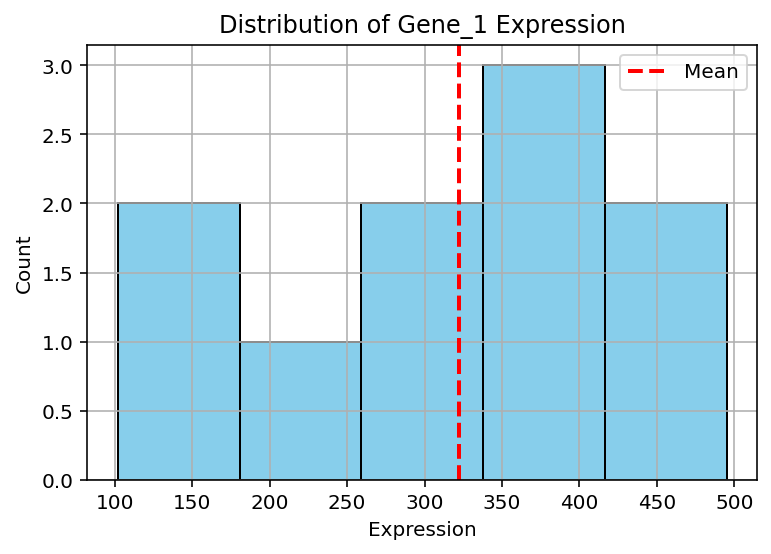
\includegraphics[keepaspectratio]{PythonIntro_SIB_files/figure-pdf/cell-22-output-1.pdf}}

\texttt{plt.show()} is what you need to do to show the plot in a popup
window. If you want to save the figure there is
\texttt{plt.savefig()}.\\
Other good practices are to close figures once they have been initiated
using \texttt{plt.close()} or \texttt{plt.clf()}.

\subsection{seaborn (sns)}\label{seaborn-sns}

seaborn usually runs on long data, so we will need to melt the pandas
dataframe from before.

\begin{Shaded}
\begin{Highlighting}[]
\CommentTok{\# melting each DF}
\ControlFlowTok{if} \StringTok{\textquotesingle{}gene\textquotesingle{}} \KeywordTok{not} \KeywordTok{in}\NormalTok{ wt1.columns:}
\NormalTok{    wt1.reset\_index(inplace}\OperatorTok{=}\VariableTok{True}\NormalTok{)}
\NormalTok{    wt1.rename(columns}\OperatorTok{=}\NormalTok{\{}\StringTok{\textquotesingle{}index\textquotesingle{}}\NormalTok{: }\StringTok{\textquotesingle{}gene\textquotesingle{}}\NormalTok{\}, inplace}\OperatorTok{=}\VariableTok{True}\NormalTok{)}
\NormalTok{wt1\_melted }\OperatorTok{=}\NormalTok{ wt1.melt(id\_vars}\OperatorTok{=}\NormalTok{[}\StringTok{\textquotesingle{}group\textquotesingle{}}\NormalTok{, }\StringTok{\textquotesingle{}id\textquotesingle{}}\NormalTok{, }\StringTok{\textquotesingle{}gene\textquotesingle{}}\NormalTok{], var\_name}\OperatorTok{=}\StringTok{\textquotesingle{}cell\textquotesingle{}}\NormalTok{, value\_name}\OperatorTok{=}\StringTok{\textquotesingle{}expression\textquotesingle{}}\NormalTok{)}

\ControlFlowTok{if} \StringTok{\textquotesingle{}gene\textquotesingle{}} \KeywordTok{not} \KeywordTok{in}\NormalTok{ wt2.columns:}
\NormalTok{    wt2.reset\_index(inplace}\OperatorTok{=}\VariableTok{True}\NormalTok{)}
\NormalTok{    wt2.rename(columns}\OperatorTok{=}\NormalTok{\{}\StringTok{\textquotesingle{}index\textquotesingle{}}\NormalTok{: }\StringTok{\textquotesingle{}gene\textquotesingle{}}\NormalTok{\}, inplace}\OperatorTok{=}\VariableTok{True}\NormalTok{)}
\NormalTok{wt2\_melted }\OperatorTok{=}\NormalTok{ wt2.melt(id\_vars}\OperatorTok{=}\NormalTok{[}\StringTok{\textquotesingle{}group\textquotesingle{}}\NormalTok{, }\StringTok{\textquotesingle{}id\textquotesingle{}}\NormalTok{, }\StringTok{\textquotesingle{}gene\textquotesingle{}}\NormalTok{], var\_name}\OperatorTok{=}\StringTok{\textquotesingle{}cell\textquotesingle{}}\NormalTok{, value\_name}\OperatorTok{=}\StringTok{\textquotesingle{}expression\textquotesingle{}}\NormalTok{)}

\ControlFlowTok{if} \StringTok{\textquotesingle{}gene\textquotesingle{}} \KeywordTok{not} \KeywordTok{in}\NormalTok{ ko1.columns:}
\NormalTok{    ko1.reset\_index(inplace}\OperatorTok{=}\VariableTok{True}\NormalTok{)}
\NormalTok{    ko1.rename(columns}\OperatorTok{=}\NormalTok{\{}\StringTok{\textquotesingle{}index\textquotesingle{}}\NormalTok{: }\StringTok{\textquotesingle{}gene\textquotesingle{}}\NormalTok{\}, inplace}\OperatorTok{=}\VariableTok{True}\NormalTok{)}
\NormalTok{ko1\_melted }\OperatorTok{=}\NormalTok{ ko1.melt(id\_vars}\OperatorTok{=}\NormalTok{[}\StringTok{\textquotesingle{}group\textquotesingle{}}\NormalTok{, }\StringTok{\textquotesingle{}id\textquotesingle{}}\NormalTok{, }\StringTok{\textquotesingle{}gene\textquotesingle{}}\NormalTok{], var\_name}\OperatorTok{=}\StringTok{\textquotesingle{}cell\textquotesingle{}}\NormalTok{, value\_name}\OperatorTok{=}\StringTok{\textquotesingle{}expression\textquotesingle{}}\NormalTok{)}

\ControlFlowTok{if} \StringTok{\textquotesingle{}gene\textquotesingle{}} \KeywordTok{not} \KeywordTok{in}\NormalTok{ ko2.columns:}
\NormalTok{    ko2.reset\_index(inplace}\OperatorTok{=}\VariableTok{True}\NormalTok{)}
\NormalTok{    ko2.rename(columns}\OperatorTok{=}\NormalTok{\{}\StringTok{\textquotesingle{}index\textquotesingle{}}\NormalTok{: }\StringTok{\textquotesingle{}gene\textquotesingle{}}\NormalTok{\}, inplace}\OperatorTok{=}\VariableTok{True}\NormalTok{)}
\NormalTok{ko2\_melted }\OperatorTok{=}\NormalTok{ ko2.melt(id\_vars}\OperatorTok{=}\NormalTok{[}\StringTok{\textquotesingle{}group\textquotesingle{}}\NormalTok{, }\StringTok{\textquotesingle{}id\textquotesingle{}}\NormalTok{, }\StringTok{\textquotesingle{}gene\textquotesingle{}}\NormalTok{], var\_name}\OperatorTok{=}\StringTok{\textquotesingle{}cell\textquotesingle{}}\NormalTok{, value\_name}\OperatorTok{=}\StringTok{\textquotesingle{}expression\textquotesingle{}}\NormalTok{)}


\CommentTok{\# Merge the DataFrames}
\NormalTok{merged\_df }\OperatorTok{=}\NormalTok{ pd.concat([wt1\_melted, wt2\_melted, ko1\_melted, ko2\_melted], ignore\_index}\OperatorTok{=}\VariableTok{True}\NormalTok{)}
\CommentTok{\#merged\_df[\textquotesingle{}gene\textquotesingle{}] = merged\_df[\textquotesingle{}gene\textquotesingle{}].apply(lambda x: \textquotesingle{}Gene\textquotesingle{} + str(int(x)))}

\BuiltInTok{print}\NormalTok{(merged\_df.head())}
\end{Highlighting}
\end{Shaded}

\begin{verbatim}
  group   id   gene   cell  expression
0    WT  WT1  Gene0  Cell0         152
1    WT  WT1  Gene1  Cell0         264
2    WT  WT1  Gene2  Cell0         307
3    WT  WT1  Gene3  Cell0          71
4    WT  WT1  Gene4  Cell0         495
\end{verbatim}

Seaborn is typically imported as \texttt{sns}.

Here, I show an example using seaborn - just requires the long form
pd.DataFrame, and you can easily plot the x and y axis based on specific
columns. Here, I am plotting a violin plot using
\texttt{sns.violinplot}, other plot types can be found
\href{https://seaborn.pydata.org/api.html}{here}.

\begin{Shaded}
\begin{Highlighting}[]
\ImportTok{import}\NormalTok{ seaborn }\ImportTok{as}\NormalTok{ sns}

\CommentTok{\# Gene1}
\NormalTok{plt.figure(figsize}\OperatorTok{=}\NormalTok{(}\DecValTok{6}\NormalTok{,}\DecValTok{4}\NormalTok{))}
\NormalTok{sns.violinplot(x}\OperatorTok{=}\StringTok{\textquotesingle{}group\textquotesingle{}}\NormalTok{, y}\OperatorTok{=}\StringTok{\textquotesingle{}expression\textquotesingle{}}\NormalTok{, data}\OperatorTok{=}\NormalTok{merged\_df[merged\_df.gene }\OperatorTok{==} \StringTok{\textquotesingle{}Gene1\textquotesingle{}}\NormalTok{], palette}\OperatorTok{=}\StringTok{\textquotesingle{}muted\textquotesingle{}}\NormalTok{)}
\NormalTok{plt.title(}\StringTok{\textquotesingle{}Gene1 Expression by Group\textquotesingle{}}\NormalTok{)}
\NormalTok{plt.show()}

\CommentTok{\#Gene3}
\NormalTok{plt.figure(figsize}\OperatorTok{=}\NormalTok{(}\DecValTok{6}\NormalTok{,}\DecValTok{4}\NormalTok{))}
\NormalTok{sns.violinplot(x}\OperatorTok{=}\StringTok{\textquotesingle{}group\textquotesingle{}}\NormalTok{, y}\OperatorTok{=}\StringTok{\textquotesingle{}expression\textquotesingle{}}\NormalTok{, data}\OperatorTok{=}\NormalTok{merged\_df[merged\_df.gene }\OperatorTok{==} \StringTok{\textquotesingle{}Gene3\textquotesingle{}}\NormalTok{], palette}\OperatorTok{=}\StringTok{\textquotesingle{}muted\textquotesingle{}}\NormalTok{)}
\NormalTok{plt.title(}\StringTok{\textquotesingle{}Gene3 Expression by Group\textquotesingle{}}\NormalTok{)}
\NormalTok{plt.show()}
\end{Highlighting}
\end{Shaded}

\begin{figure}

\begin{minipage}{0.50\linewidth}

\begin{figure}[H]

{\centering \pandocbounded{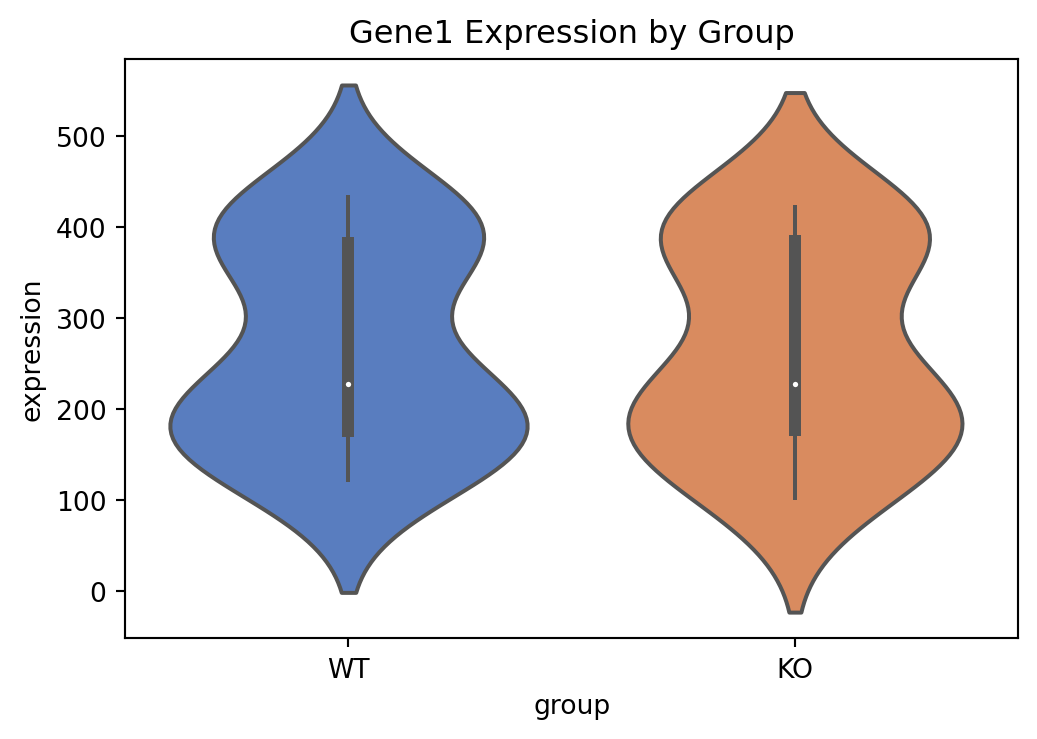
\includegraphics[keepaspectratio]{PythonIntro_SIB_files/figure-pdf/cell-24-output-1.pdf}}

}

\subcaption{Violin plot: gene 1}

\end{figure}%

\end{minipage}%
%
\begin{minipage}{0.50\linewidth}

\begin{figure}[H]

{\centering \pandocbounded{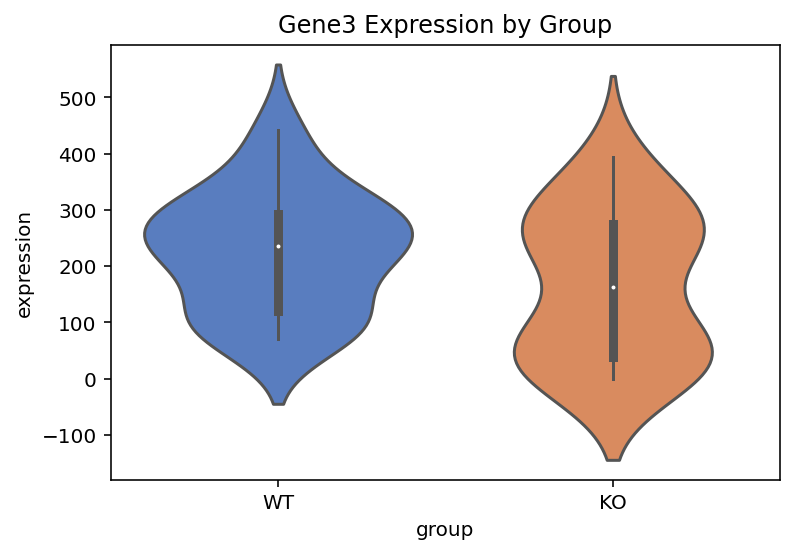
\includegraphics[keepaspectratio]{PythonIntro_SIB_files/figure-pdf/cell-24-output-2.pdf}}

}

\subcaption{Violin plot gene 3}

\end{figure}%

\end{minipage}%

\end{figure}%

In this example, I am layering using seaborn - plotting a swarmplot
above the catplot. I store the catplot in the variable g, I then plot
the swarmplot on the same axes by using \texttt{ax=g.ax}.

\begin{Shaded}
\begin{Highlighting}[]
\ImportTok{import}\NormalTok{ seaborn }\ImportTok{as}\NormalTok{ sns}

\CommentTok{\# Gene2}
\NormalTok{g }\OperatorTok{=}\NormalTok{ sns.catplot(data}\OperatorTok{=}\NormalTok{merged\_df[merged\_df.gene }\OperatorTok{==} \StringTok{\textquotesingle{}Gene2\textquotesingle{}}\NormalTok{], x}\OperatorTok{=}\StringTok{"group"}\NormalTok{, y}\OperatorTok{=}\StringTok{"expression"}\NormalTok{,}
\NormalTok{                kind}\OperatorTok{=}\StringTok{"violin"}\NormalTok{, color}\OperatorTok{=}\StringTok{".9"}\NormalTok{, inner}\OperatorTok{=}\VariableTok{None}\NormalTok{, height}\OperatorTok{=}\DecValTok{4}\NormalTok{, aspect}\OperatorTok{=}\FloatTok{1.5}\NormalTok{)}
\NormalTok{sns.swarmplot(data}\OperatorTok{=}\NormalTok{merged\_df[merged\_df.gene }\OperatorTok{==} \StringTok{\textquotesingle{}Gene2\textquotesingle{}}\NormalTok{], x}\OperatorTok{=}\StringTok{"group"}\NormalTok{, y}\OperatorTok{=}\StringTok{"expression"}\NormalTok{, size}\OperatorTok{=}\DecValTok{3}\NormalTok{, ax}\OperatorTok{=}\NormalTok{g.ax)}
\NormalTok{g.ax.set\_title(}\StringTok{\textquotesingle{}Gene2 Expression by Group\textquotesingle{}}\NormalTok{)}
\NormalTok{plt.show()}

\CommentTok{\# gene7}
\NormalTok{g }\OperatorTok{=}\NormalTok{ sns.catplot(data}\OperatorTok{=}\NormalTok{merged\_df[merged\_df.gene }\OperatorTok{==} \StringTok{\textquotesingle{}Gene7\textquotesingle{}}\NormalTok{], x}\OperatorTok{=}\StringTok{"group"}\NormalTok{, y}\OperatorTok{=}\StringTok{"expression"}\NormalTok{,}
\NormalTok{                kind}\OperatorTok{=}\StringTok{"violin"}\NormalTok{, color}\OperatorTok{=}\StringTok{".9"}\NormalTok{, inner}\OperatorTok{=}\VariableTok{None}\NormalTok{, height}\OperatorTok{=}\DecValTok{4}\NormalTok{, aspect}\OperatorTok{=}\FloatTok{1.5}\NormalTok{)}
\NormalTok{sns.swarmplot(data}\OperatorTok{=}\NormalTok{merged\_df[merged\_df.gene }\OperatorTok{==} \StringTok{\textquotesingle{}Gene7\textquotesingle{}}\NormalTok{], x}\OperatorTok{=}\StringTok{"group"}\NormalTok{, y}\OperatorTok{=}\StringTok{"expression"}\NormalTok{, size}\OperatorTok{=}\DecValTok{3}\NormalTok{, ax}\OperatorTok{=}\NormalTok{g.ax)}
\NormalTok{g.ax.set\_title(}\StringTok{\textquotesingle{}Gene7 Expression by Group\textquotesingle{}}\NormalTok{)}
\NormalTok{plt.show()}


\CommentTok{\# you can access the data in the sns.FacetGrid object (variable g in my script) by calling g.data}
\end{Highlighting}
\end{Shaded}

\begin{figure}

\begin{minipage}{0.50\linewidth}

\begin{figure}[H]

{\centering \pandocbounded{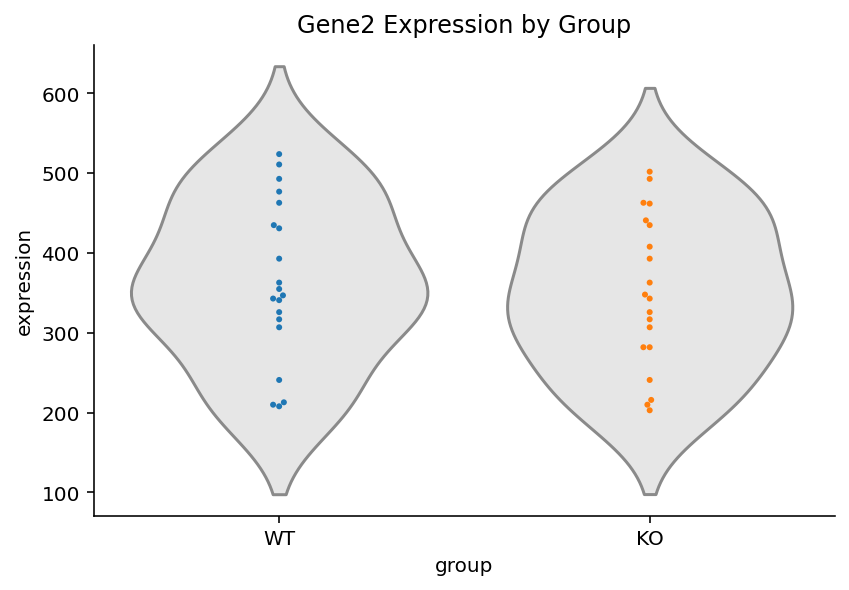
\includegraphics[keepaspectratio]{PythonIntro_SIB_files/figure-pdf/cell-25-output-1.pdf}}

}

\subcaption{Violin plot: gene 2}

\end{figure}%

\end{minipage}%
%
\begin{minipage}{0.50\linewidth}

\begin{figure}[H]

{\centering \pandocbounded{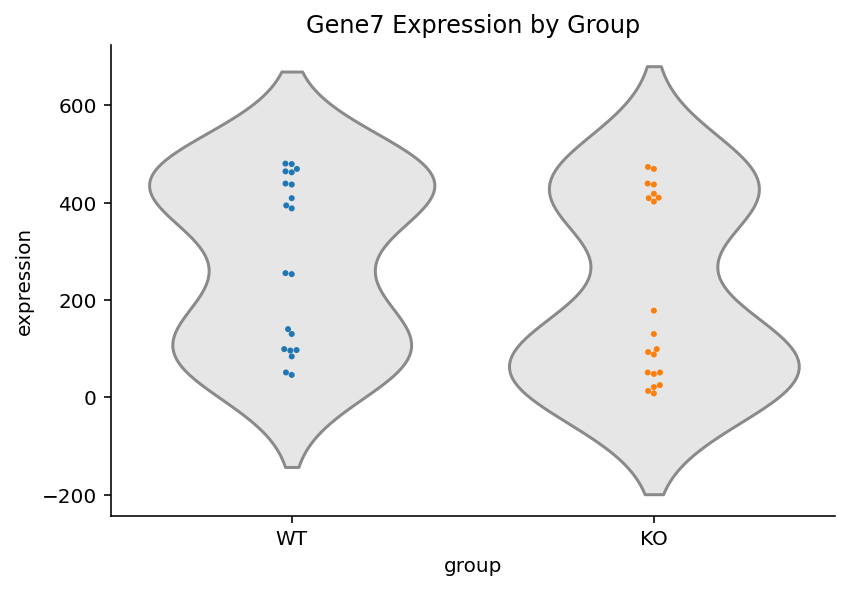
\includegraphics[keepaspectratio]{PythonIntro_SIB_files/figure-pdf/cell-25-output-2.pdf}}

}

\subcaption{Violin plot gene 7}

\end{figure}%

\end{minipage}%

\end{figure}%

In the example below I use \texttt{sns.scatterplot} to plot a volcano
plot. I generate some fake data.\\
I use seaborn for the scatter plot, and then layer on top of it using
\texttt{matplotlib.pyplot} (\texttt{plt}).

\begin{Shaded}
\begin{Highlighting}[]
\CommentTok{\# creating fake log2 fold change and p{-}value data}
\NormalTok{volcano\_data }\OperatorTok{=}\NormalTok{ pd.DataFrame(\{}
    \CommentTok{\#\textquotesingle{}gene\textquotesingle{}: [\textquotesingle{}Gene0\textquotesingle{}, \textquotesingle{}Gene1\textquotesingle{}, \textquotesingle{}Gene2\textquotesingle{}, \textquotesingle{}Gene3\textquotesingle{}, \textquotesingle{}Gene4\textquotesingle{}, \textquotesingle{}Gene5\textquotesingle{}, \textquotesingle{}Gene6\textquotesingle{}, \textquotesingle{}Gene7\textquotesingle{}, \textquotesingle{}Gene8\textquotesingle{}, \textquotesingle{}Gene9\textquotesingle{}],}
    \StringTok{\textquotesingle{}log2FC\textquotesingle{}}\NormalTok{: np.random.randn(}\DecValTok{1000}\NormalTok{),  }\CommentTok{\# Random fold changes}
    \StringTok{\textquotesingle{}pval\textquotesingle{}}\NormalTok{: np.random.rand(}\DecValTok{1000}\NormalTok{)  }\CommentTok{\# Random p{-}values}
\NormalTok{\})}

\CommentTok{\# calculating {-}log10(p{-}value)}
\NormalTok{volcano\_data[}\StringTok{\textquotesingle{}{-}log10(pval)\textquotesingle{}}\NormalTok{] }\OperatorTok{=} \OperatorTok{{-}}\NormalTok{np.log10(volcano\_data[}\StringTok{\textquotesingle{}pval\textquotesingle{}}\NormalTok{])}

\NormalTok{plt.figure(figsize}\OperatorTok{=}\NormalTok{(}\DecValTok{6}\NormalTok{,}\DecValTok{5}\NormalTok{))}
\NormalTok{sns.scatterplot(data}\OperatorTok{=}\NormalTok{volcano\_data, x}\OperatorTok{=}\StringTok{\textquotesingle{}log2FC\textquotesingle{}}\NormalTok{, y}\OperatorTok{=}\StringTok{\textquotesingle{}{-}log10(pval)\textquotesingle{}}\NormalTok{, color}\OperatorTok{=}\StringTok{\textquotesingle{}purple\textquotesingle{}}\NormalTok{)}
\NormalTok{plt.axhline(y}\OperatorTok{=}\FloatTok{1.3}\NormalTok{, color}\OperatorTok{=}\StringTok{\textquotesingle{}red\textquotesingle{}}\NormalTok{, linestyle}\OperatorTok{=}\StringTok{\textquotesingle{}dashed\textquotesingle{}}\NormalTok{)  }\CommentTok{\# threshold line for p{-}value = 0.05}
\NormalTok{plt.axvline(x}\OperatorTok{=}\DecValTok{0}\NormalTok{, color}\OperatorTok{=}\StringTok{\textquotesingle{}black\textquotesingle{}}\NormalTok{, linestyle}\OperatorTok{=}\StringTok{\textquotesingle{}dotted\textquotesingle{}}\NormalTok{)}
\NormalTok{plt.title(}\StringTok{\textquotesingle{}Volcano Plot (Mock Example)\textquotesingle{}}\NormalTok{)}
\NormalTok{plt.xlabel(}\StringTok{\textquotesingle{}Log2 Fold Change\textquotesingle{}}\NormalTok{)}
\NormalTok{plt.ylabel(}\StringTok{\textquotesingle{}{-}Log10(p{-}value)\textquotesingle{}}\NormalTok{)}
\NormalTok{plt.show()}
\end{Highlighting}
\end{Shaded}

\pandocbounded{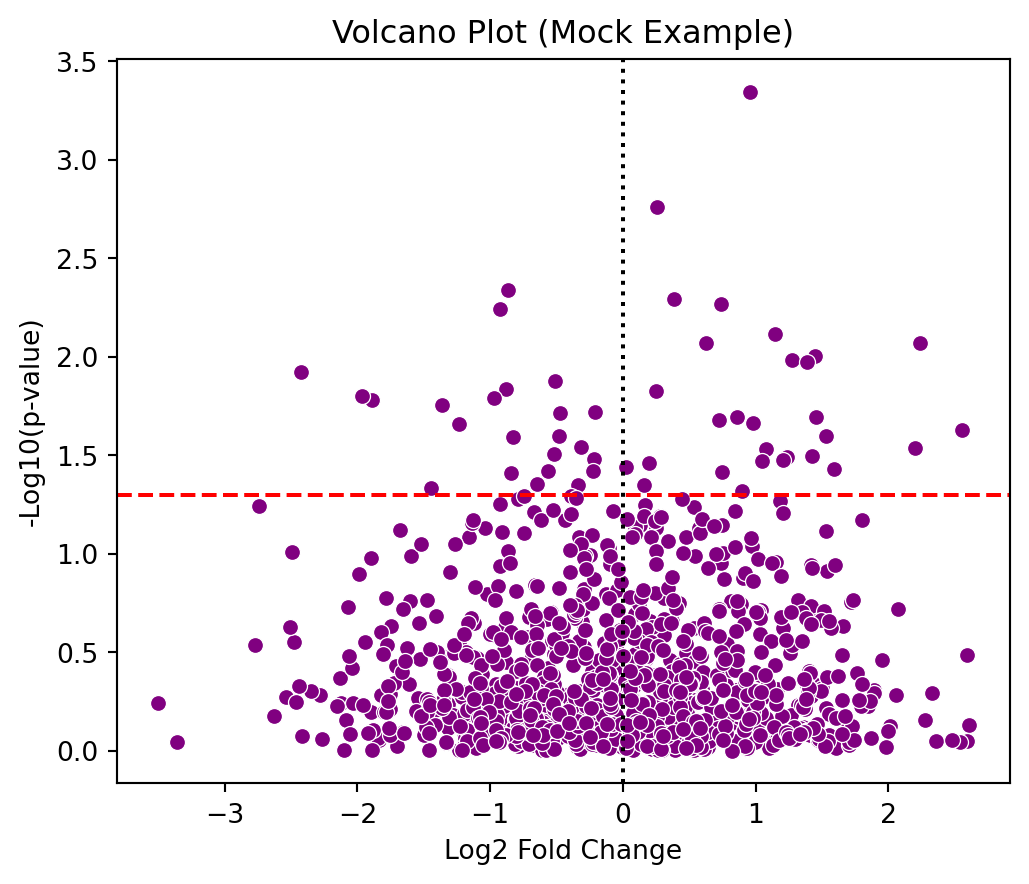
\includegraphics[keepaspectratio]{PythonIntro_SIB_files/figure-pdf/cell-26-output-1.pdf}}

\subsection{plotly}\label{plotly}

Plotly exists in R as well, and is good for interactivity - widget-like
plots. You can hover over points and filter points by clicking on the
legend.

plotly express functions are not too dissimilar to using seabron - in
the example below I use \texttt{px.strip} to generate a strip plot. It
requires long data format \texttt{pd.DataFrame}, and you plot simply by
putting the columns you want to plot under x and y (columns group and
expression, respectively). The colour of each point is based on the
column cell.

\begin{Shaded}
\begin{Highlighting}[]
\ImportTok{import}\NormalTok{ plotly.express }\ImportTok{as}\NormalTok{ px}

\CommentTok{\# Plotly: Strip Plot (interactive)}
\NormalTok{fig }\OperatorTok{=}\NormalTok{ px.strip(merged\_df[merged\_df.gene }\OperatorTok{==} \StringTok{\textquotesingle{}Gene3\textquotesingle{}}\NormalTok{], x}\OperatorTok{=}\StringTok{\textquotesingle{}group\textquotesingle{}}\NormalTok{, y}\OperatorTok{=}\StringTok{\textquotesingle{}expression\textquotesingle{}}\NormalTok{, color}\OperatorTok{=}\StringTok{\textquotesingle{}cell\textquotesingle{}}\NormalTok{, stripmode}\OperatorTok{=}\StringTok{\textquotesingle{}overlay\textquotesingle{}}\NormalTok{, title}\OperatorTok{=}\StringTok{\textquotesingle{}Gene Expression by Cell (WT vs KO)\textquotesingle{}}\NormalTok{)}
\NormalTok{fig.show()}

\CommentTok{\# the variable fig is a plotly.graph\_objects.Figure}
\end{Highlighting}
\end{Shaded}

\begin{verbatim}
Unable to display output for mime type(s): text/html
\end{verbatim}

\begin{verbatim}
Unable to display output for mime type(s): text/html
\end{verbatim}

\section{TIP 11: You can do your statistical tests in python using
scipy.stats or
statsmodels}\label{tip-11-you-can-do-your-statistical-tests-in-python-using-scipy.stats-or-statsmodels}

R is known for being able to carry out stats tests, but through packages
such as statsmodels and scipy.stats, we have access to many statistical
tests that you need for scientific studies.

I will show you some examples, these tests are shown only for
demonstration; there's no real hypothesis being tested.

\subsection{GLM}\label{glm}

\begin{Shaded}
\begin{Highlighting}[]
\ImportTok{import}\NormalTok{ statsmodels.api }\ImportTok{as}\NormalTok{ sm}


\CommentTok{\#merged\_df[\textquotesingle{}group\_binary\textquotesingle{}] = merged\_df[\textquotesingle{}group\textquotesingle{}].apply(lambda x: 1 if x == \textquotesingle{}KO\textquotesingle{} else 0) \# converting KO/WT to binary 0/1.}

\CommentTok{\# for this example, we will just put gene expression as a continuous response}
\NormalTok{X }\OperatorTok{=}\NormalTok{ pd.get\_dummies(merged\_df[}\StringTok{\textquotesingle{}group\textquotesingle{}}\NormalTok{], drop\_first}\OperatorTok{=}\VariableTok{True}\NormalTok{)  }\CommentTok{\# one{-}hot encoding for group variable}
\NormalTok{X }\OperatorTok{=}\NormalTok{ sm.add\_constant(X)  }\CommentTok{\# add intercept}
\NormalTok{y }\OperatorTok{=}\NormalTok{ merged\_df[}\StringTok{\textquotesingle{}expression\textquotesingle{}}\NormalTok{]}

\CommentTok{\# Fit GLM}
\NormalTok{model }\OperatorTok{=}\NormalTok{ sm.GLM(y, X, family}\OperatorTok{=}\NormalTok{sm.families.Gaussian()).fit()}

\CommentTok{\# Show the results}
\BuiltInTok{print}\NormalTok{(model.summary())}
\end{Highlighting}
\end{Shaded}

\begin{verbatim}
                 Generalized Linear Model Regression Results                  
==============================================================================
Dep. Variable:             expression   No. Observations:                  400
Model:                            GLM   Df Residuals:                      398
Model Family:                Gaussian   Df Model:                            1
Link Function:               identity   Scale:                          17963.
Method:                          IRLS   Log-Likelihood:                -2525.8
Date:                Wed, 30 Apr 2025   Deviance:                   7.1492e+06
Time:                        15:38:29   Pearson chi2:                 7.15e+06
No. Iterations:                     3   Pseudo R-squ. (CS):           0.002870
Covariance Type:            nonrobust                                         
==============================================================================
                 coef    std err          z      P>|z|      [0.025      0.975]
------------------------------------------------------------------------------
const        269.2350      9.477     28.409      0.000     250.660     287.810
WT            14.3400     13.403      1.070      0.285     -11.928      40.608
==============================================================================
\end{verbatim}

\subsection{T-test}\label{t-test}

\begin{Shaded}
\begin{Highlighting}[]
\ImportTok{from}\NormalTok{ scipy }\ImportTok{import}\NormalTok{ stats}

\CommentTok{\# two conditions WT vs KO, different in expression}
\NormalTok{ko\_expr }\OperatorTok{=}\NormalTok{ merged\_df[merged\_df[}\StringTok{\textquotesingle{}group\textquotesingle{}}\NormalTok{] }\OperatorTok{==} \StringTok{\textquotesingle{}KO\textquotesingle{}}\NormalTok{][}\StringTok{\textquotesingle{}expression\textquotesingle{}}\NormalTok{]}
\NormalTok{wt\_expr }\OperatorTok{=}\NormalTok{ merged\_df[merged\_df[}\StringTok{\textquotesingle{}group\textquotesingle{}}\NormalTok{] }\OperatorTok{==} \StringTok{\textquotesingle{}WT\textquotesingle{}}\NormalTok{][}\StringTok{\textquotesingle{}expression\textquotesingle{}}\NormalTok{]}

\CommentTok{\# performing two{-}sample t{-}test}
\NormalTok{t\_stat, p\_value }\OperatorTok{=}\NormalTok{ stats.ttest\_ind(ko\_expr, wt\_expr)}

\BuiltInTok{print}\NormalTok{(}\SpecialStringTok{f"T{-}statistic: }\SpecialCharTok{\{}\NormalTok{t\_stat}\SpecialCharTok{\}}\SpecialStringTok{, P{-}value: }\SpecialCharTok{\{}\NormalTok{p\_value}\SpecialCharTok{\}}\SpecialStringTok{"}\NormalTok{)}
\end{Highlighting}
\end{Shaded}

\begin{verbatim}
T-statistic: -1.069947991397797, P-value: 0.2852911632028579
\end{verbatim}

\subsection{Chi2 test}\label{chi2-test}

\begin{Shaded}
\begin{Highlighting}[]
\CommentTok{\# categorising gene expression into \textquotesingle{}high\textquotesingle{} or \textquotesingle{}low\textquotesingle{} based on median expression}
\NormalTok{median\_expr }\OperatorTok{=}\NormalTok{ merged\_df[}\StringTok{\textquotesingle{}expression\textquotesingle{}}\NormalTok{].median()}
\NormalTok{merged\_df[}\StringTok{\textquotesingle{}expr\_category\textquotesingle{}}\NormalTok{] }\OperatorTok{=}\NormalTok{ merged\_df[}\StringTok{\textquotesingle{}expression\textquotesingle{}}\NormalTok{].}\BuiltInTok{apply}\NormalTok{(}\KeywordTok{lambda}\NormalTok{ x: }\StringTok{\textquotesingle{}high\textquotesingle{}} \ControlFlowTok{if}\NormalTok{ x }\OperatorTok{\textgreater{}}\NormalTok{ median\_expr }\ControlFlowTok{else} \StringTok{\textquotesingle{}low\textquotesingle{}}\NormalTok{)}

\CommentTok{\# creating a contingency table for chisq test}
\NormalTok{contingency }\OperatorTok{=}\NormalTok{ pd.crosstab(merged\_df[}\StringTok{\textquotesingle{}expr\_category\textquotesingle{}}\NormalTok{], merged\_df[}\StringTok{\textquotesingle{}group\textquotesingle{}}\NormalTok{])}

\CommentTok{\# performing the Chi{-}Squared test}
\NormalTok{chi2, p\_val, dof, expected }\OperatorTok{=}\NormalTok{ stats.chi2\_contingency(contingency)}

\BuiltInTok{print}\NormalTok{(}\SpecialStringTok{f"Chi{-}Squared: }\SpecialCharTok{\{}\NormalTok{chi2}\SpecialCharTok{\}}\SpecialStringTok{, P{-}value: }\SpecialCharTok{\{}\NormalTok{p\_val}\SpecialCharTok{\}}\SpecialStringTok{"}\NormalTok{)}
\end{Highlighting}
\end{Shaded}

\begin{verbatim}
Chi-Squared: 0.4900490049004901, P-value: 0.4839054452991407
\end{verbatim}

\subsection{ANOVA}\label{anova}

\begin{Shaded}
\begin{Highlighting}[]
\CommentTok{\# performing ANOVA on expression values grouped by the \textquotesingle{}group\textquotesingle{} column}
\NormalTok{group1 }\OperatorTok{=}\NormalTok{ merged\_df[merged\_df[}\StringTok{\textquotesingle{}group\textquotesingle{}}\NormalTok{] }\OperatorTok{==} \StringTok{\textquotesingle{}WT\textquotesingle{}}\NormalTok{][}\StringTok{\textquotesingle{}expression\textquotesingle{}}\NormalTok{]}
\NormalTok{group2 }\OperatorTok{=}\NormalTok{ merged\_df[merged\_df[}\StringTok{\textquotesingle{}group\textquotesingle{}}\NormalTok{] }\OperatorTok{==} \StringTok{\textquotesingle{}KO\textquotesingle{}}\NormalTok{][}\StringTok{\textquotesingle{}expression\textquotesingle{}}\NormalTok{]}

\NormalTok{f\_stat, p\_val }\OperatorTok{=}\NormalTok{ stats.f\_oneway(group1, group2)}
\BuiltInTok{print}\NormalTok{(}\SpecialStringTok{f"ANOVA F{-}statistic: }\SpecialCharTok{\{}\NormalTok{f\_stat}\SpecialCharTok{\}}\SpecialStringTok{, P{-}value: }\SpecialCharTok{\{}\NormalTok{p\_val}\SpecialCharTok{\}}\SpecialStringTok{"}\NormalTok{)}
\end{Highlighting}
\end{Shaded}

\begin{verbatim}
ANOVA F-statistic: 1.144788704296184, P-value: 0.28529116320296
\end{verbatim}

\subsection{Running correction on multiple
testing}\label{running-correction-on-multiple-testing}

\begin{Shaded}
\begin{Highlighting}[]
\ImportTok{import}\NormalTok{ pandas }\ImportTok{as}\NormalTok{ pd}
\ImportTok{import}\NormalTok{ scipy.stats }\ImportTok{as}\NormalTok{ stats}
\ImportTok{from}\NormalTok{ statsmodels.stats.multitest }\ImportTok{import}\NormalTok{ multipletests}


\CommentTok{\# creating a list to store p{-}values {-} we will run multiple test correction}
\NormalTok{p\_values }\OperatorTok{=}\NormalTok{ []}

\CommentTok{\# iterating over each gene (rows of the dataframe) to get expression for KO and WT}
\ControlFlowTok{for}\NormalTok{ g }\KeywordTok{in}\NormalTok{ merged\_df.gene.unique():}
    \CommentTok{\# getting expression data for the gene in both KO and WT groups}
\NormalTok{    ko\_expr }\OperatorTok{=}\NormalTok{ merged\_df[(merged\_df.gene }\OperatorTok{==}\NormalTok{ g) }\OperatorTok{\&}\NormalTok{ (merged\_df.group }\OperatorTok{==} \StringTok{\textquotesingle{}KO\textquotesingle{}}\NormalTok{)][}\StringTok{\textquotesingle{}expression\textquotesingle{}}\NormalTok{].to\_numpy()}
\NormalTok{    wt\_expr }\OperatorTok{=}\NormalTok{ merged\_df[(merged\_df.gene }\OperatorTok{==}\NormalTok{ g) }\OperatorTok{\&}\NormalTok{ (merged\_df.group }\OperatorTok{==} \StringTok{\textquotesingle{}WT\textquotesingle{}}\NormalTok{)][}\StringTok{\textquotesingle{}expression\textquotesingle{}}\NormalTok{].to\_numpy()}

    \CommentTok{\# performing two{-}sample t{-}test on each gene expression data}
\NormalTok{    t\_stat, p\_val }\OperatorTok{=}\NormalTok{ stats.ttest\_ind(ko\_expr, wt\_expr, equal\_var}\OperatorTok{=}\VariableTok{False}\NormalTok{)}
\NormalTok{    p\_values.append(p\_val)}

\CommentTok{\# Now we will apply multiple testing correction to the p{-}values using Benjamini{-}Hochberg (FDR) method, other methods such as Bonferroni are available}
\NormalTok{reject, corrected\_pvals, \_, \_ }\OperatorTok{=}\NormalTok{ multipletests(p\_values, alpha}\OperatorTok{=}\FloatTok{0.05}\NormalTok{, method}\OperatorTok{=}\StringTok{\textquotesingle{}fdr\_bh\textquotesingle{}}\NormalTok{)}

\CommentTok{\# Create a dataframe to view the results}
\NormalTok{results }\OperatorTok{=}\NormalTok{ pd.DataFrame(\{}
    \StringTok{\textquotesingle{}gene\textquotesingle{}}\NormalTok{: merged\_df.gene.unique(),}
    \StringTok{\textquotesingle{}p{-}value\textquotesingle{}}\NormalTok{: p\_values,}
    \StringTok{\textquotesingle{}corrected p{-}value\textquotesingle{}}\NormalTok{: corrected\_pvals,}
    \StringTok{\textquotesingle{}reject null hypothesis\textquotesingle{}}\NormalTok{: reject}
\NormalTok{\})}

\BuiltInTok{print}\NormalTok{(results)}
\end{Highlighting}
\end{Shaded}

\begin{verbatim}
    gene   p-value  corrected p-value  reject null hypothesis
0  Gene0  0.935963           0.995188                   False
1  Gene1  0.951398           0.995188                   False
2  Gene2  0.673559           0.995188                   False
3  Gene3  0.106674           0.995188                   False
4  Gene4  0.816119           0.995188                   False
5  Gene5  0.864392           0.995188                   False
6  Gene6  0.995188           0.995188                   False
7  Gene7  0.224214           0.995188                   False
8  Gene8  0.886540           0.995188                   False
9  Gene9  0.667638           0.995188                   False
\end{verbatim}

\section{TIP 12: You can parallelise your code using
multiprocessing}\label{tip-12-you-can-parallelise-your-code-using-multiprocessing}

\begin{Shaded}
\begin{Highlighting}[]
\ImportTok{import}\NormalTok{ time}
\ImportTok{import}\NormalTok{ multiprocessing}


\KeywordTok{def}\NormalTok{ calculate\_square(number):}
    \CommentTok{\textquotesingle{}\textquotesingle{}\textquotesingle{}}
\CommentTok{    function to calculate square of a number (CPU{-}bound task)}
\CommentTok{    \textquotesingle{}\textquotesingle{}\textquotesingle{}}
    \ControlFlowTok{return}\NormalTok{ number }\OperatorTok{*}\NormalTok{ number}


\KeywordTok{def}\NormalTok{ parallel\_square(numbers):}
    \CommentTok{\textquotesingle{}\textquotesingle{}\textquotesingle{}}
\CommentTok{    function to run the calculation in parallel using multiple processes}
\CommentTok{    \textquotesingle{}\textquotesingle{}\textquotesingle{}}
    \CommentTok{\# you need to create a pool of worker processes}
    \ControlFlowTok{with}\NormalTok{ multiprocessing.Pool(processes}\OperatorTok{=}\NormalTok{multiprocessing.cpu\_count()) }\ImportTok{as}\NormalTok{ pool: }\CommentTok{\# line that lets you access your cpus to run script}
\NormalTok{        result }\OperatorTok{=}\NormalTok{ pool.}\BuiltInTok{map}\NormalTok{(calculate\_square, numbers)}
    \ControlFlowTok{return}\NormalTok{ result}

\KeywordTok{def}\NormalTok{ single\_threaded\_square(numbers):}
    \CommentTok{\textquotesingle{}\textquotesingle{}\textquotesingle{}}
\CommentTok{    single{-}threaded version: Calculating squares sequentially}
\CommentTok{    \textquotesingle{}\textquotesingle{}\textquotesingle{}}
\NormalTok{    result }\OperatorTok{=}\NormalTok{ []}
    \ControlFlowTok{for}\NormalTok{ number }\KeywordTok{in}\NormalTok{ numbers:}
\NormalTok{        result.append(calculate\_square(number))}
    \ControlFlowTok{return}\NormalTok{ result}

\ControlFlowTok{if} \VariableTok{\_\_name\_\_} \OperatorTok{==} \StringTok{"\_\_main\_\_"}\NormalTok{:}
\NormalTok{    numbers }\OperatorTok{=}\NormalTok{ [x }\ControlFlowTok{for}\NormalTok{ x }\KeywordTok{in} \BuiltInTok{range}\NormalTok{(}\DecValTok{1}\NormalTok{, }\DecValTok{10000001}\NormalTok{)]  }\CommentTok{\# 10 million numbers}
    
    \CommentTok{\# measuring the time for the single{-}threaded execution}
\NormalTok{    start\_time }\OperatorTok{=}\NormalTok{ time.time()}
\NormalTok{    single\_result }\OperatorTok{=}\NormalTok{ single\_threaded\_square(numbers)}
\NormalTok{    single\_thread\_time }\OperatorTok{=}\NormalTok{ time.time() }\OperatorTok{{-}}\NormalTok{ start\_time}
    \BuiltInTok{print}\NormalTok{(}\SpecialStringTok{f"Single{-}threaded time: }\SpecialCharTok{\{}\NormalTok{single\_thread\_time}\SpecialCharTok{:.2f\}}\SpecialStringTok{ seconds"}\NormalTok{)}
    
    \CommentTok{\# measuring the time for the parallel execution}
\NormalTok{    start\_time }\OperatorTok{=}\NormalTok{ time.time()}
\NormalTok{    parallel\_result }\OperatorTok{=}\NormalTok{ parallel\_square(numbers)}
\NormalTok{    parallel\_time }\OperatorTok{=}\NormalTok{ time.time() }\OperatorTok{{-}}\NormalTok{ start\_time}
    \BuiltInTok{print}\NormalTok{(}\SpecialStringTok{f"Parallel execution time: }\SpecialCharTok{\{}\NormalTok{parallel\_time}\SpecialCharTok{:.2f\}}\SpecialStringTok{ seconds"}\NormalTok{)}
    
    \CommentTok{\# comparing results to make sure they are the same}
    \BuiltInTok{print}\NormalTok{(}\SpecialStringTok{f"Do the results match? }\SpecialCharTok{\{}\StringTok{\textquotesingle{}Yes\textquotesingle{}} \ControlFlowTok{if}\NormalTok{ single\_result }\OperatorTok{==}\NormalTok{ parallel\_result }\ControlFlowTok{else} \StringTok{\textquotesingle{}No\textquotesingle{}}\SpecialCharTok{\}}\SpecialStringTok{"}\NormalTok{)}
\end{Highlighting}
\end{Shaded}

\begin{verbatim}
Single-threaded time: 1.22 seconds
Parallel execution time: 1.87 seconds
Do the results match? Yes
\end{verbatim}

\section{TIP 13: You can generate pipelines using bash/python/r with
Snakemake}\label{tip-13-you-can-generate-pipelines-using-bashpythonr-with-snakemake}

show basic snakemake document with three rules: cellranger {[}bash{]},
preprocessing {[}python{]}, plotting {[}r{]}

\begin{Shaded}
\begin{Highlighting}[]
\CommentTok{\# Snakefile}

\CommentTok{\# Define the rule for Cell Ranger processing}
\NormalTok{rule cellranger:}
    \BuiltInTok{input}\NormalTok{:}
\NormalTok{        r1}\OperatorTok{=}\StringTok{"data/}\SpecialCharTok{\{sample\}}\StringTok{\_R1.fastq.gz"}\NormalTok{,}
\NormalTok{        r2}\OperatorTok{=}\StringTok{"data/}\SpecialCharTok{\{sample\}}\StringTok{\_R2.fastq.gz"}
\NormalTok{    output:}
        \CommentTok{"output/cellranger\_output/\{sample\}/filtered\_feature\_bc\_matrix"}
\NormalTok{    shell:}
        \CommentTok{"cellranger count {-}{-}id=\{wildcards.sample\} "}
        \CommentTok{"{-}{-}fastqs=\{input.r1\},\{input.r2\} "}
        \CommentTok{"{-}{-}transcriptome=/path/to/refdata{-}cellranger{-}mm10{-}3.0.0 "}
        \CommentTok{"{-}{-}sample=\{wildcards.sample\}"}

\CommentTok{\# Define the rule for Python data processing}
\NormalTok{rule process\_data:}
    \BuiltInTok{input}\NormalTok{:}
        \CommentTok{"output/cellranger\_output/\{sample\}/filtered\_feature\_bc\_matrix/matrix.mtx"}
\NormalTok{    output:}
        \CommentTok{"output/analysis\_results/\{sample\}\_processed.csv"}
\NormalTok{    script:}
        \CommentTok{"scripts/process\_data.py"}

\CommentTok{\# Define the rule for generating plots using R}
\NormalTok{rule plot\_data:}
    \BuiltInTok{input}\NormalTok{:}
        \CommentTok{"output/analysis\_results/\{sample\}\_processed.csv"}
\NormalTok{    output:}
        \CommentTok{"output/analysis\_results/\{sample\}\_plot.png"}
\NormalTok{    script:}
        \CommentTok{"scripts/plot\_data.R"}
\end{Highlighting}
\end{Shaded}

run workflow with \texttt{snakemake\ -\/-cores\ 4\ -s\ Snakefile}

\section{TIP 14: Use type hinting to write clearly usable functions and
unit testing to ensure your programmes work as
expected.}\label{tip-14-use-type-hinting-to-write-clearly-usable-functions-and-unit-testing-to-ensure-your-programmes-work-as-expected.}

In the example below, it shows the function normalise requires the
argument \texttt{x} and this should be of type \texttt{np.ndarray}, and
the \texttt{-\textgreater{}\ np.ndarray}, shows the expected output
should be of type \texttt{np.ndarray} - helping you or someone else know
what to expect from this function.

\begin{Shaded}
\begin{Highlighting}[]
\KeywordTok{def}\NormalTok{ normalise(x: np.ndarray) }\OperatorTok{{-}\textgreater{}}\NormalTok{ np.ndarray:}
    \ControlFlowTok{return}\NormalTok{ x }\OperatorTok{/}\NormalTok{ x.}\BuiltInTok{sum}\NormalTok{()}
\end{Highlighting}
\end{Shaded}

Other common types: \texttt{int}, \texttt{float}, \texttt{list},
\texttt{tuple}, \texttt{range}, \texttt{str}, \texttt{set},
\texttt{dict}, \texttt{bool}, \texttt{NoneType}, \texttt{pd.Series},
\texttt{pd.DataFrame}, \texttt{np.ndarray}, \texttt{np.int64},
\texttt{np.float64}, \texttt{sc.AnnData}.

Unit testing is a crucial practice, especially when your code is
intended for use by others or will be reused in the future. It involves
writing small tests that check whether individual functions behave as
expected given specific inputs. These tests help catch bugs early,
document expected behavior, and ensure that future changes don't break
existing functionality. Implementing unit tests improves code
reliability and maintainability. You can use \texttt{unittest} or
\texttt{pytest} for this.

\begin{Shaded}
\begin{Highlighting}[]
\ImportTok{import}\NormalTok{ unittest}
\ImportTok{import}\NormalTok{ numpy }\ImportTok{as}\NormalTok{ np}

\KeywordTok{class}\NormalTok{ TestNormaliseFunction(unittest.TestCase):}

    \KeywordTok{def}\NormalTok{ test\_normalise\_single\_dimension(}\VariableTok{self}\NormalTok{):}
        \CommentTok{"""Test normalization of a 1D array."""}
\NormalTok{        x }\OperatorTok{=}\NormalTok{ np.array([}\DecValTok{1}\NormalTok{, }\DecValTok{2}\NormalTok{, }\DecValTok{3}\NormalTok{])}
\NormalTok{        expected }\OperatorTok{=}\NormalTok{ np.array([}\FloatTok{0.16666667}\NormalTok{, }\FloatTok{0.33333333}\NormalTok{, }\FloatTok{0.5}\NormalTok{])  }\CommentTok{\# sum = 6, so divide each element by 6}
\NormalTok{        result }\OperatorTok{=}\NormalTok{ normalise(x)}
\NormalTok{        np.testing.assert\_array\_almost\_equal(result, expected, decimal}\OperatorTok{=}\DecValTok{8}\NormalTok{)}
    
    \KeywordTok{def}\NormalTok{ test\_normalise\_multiple\_dimension(}\VariableTok{self}\NormalTok{):}
        \CommentTok{"""Test normalization of a 2D array."""}
\NormalTok{        x }\OperatorTok{=}\NormalTok{ np.array([[}\DecValTok{1}\NormalTok{, }\DecValTok{2}\NormalTok{], [}\DecValTok{3}\NormalTok{, }\DecValTok{4}\NormalTok{]])}
\NormalTok{        expected }\OperatorTok{=}\NormalTok{ np.array([[}\FloatTok{0.1}\NormalTok{, }\FloatTok{0.2}\NormalTok{], [}\FloatTok{0.3}\NormalTok{, }\FloatTok{0.4}\NormalTok{]])  }\CommentTok{\# sum = 10, divide each element by 10}
\NormalTok{        result }\OperatorTok{=}\NormalTok{ normalise(x)}
\NormalTok{        np.testing.assert\_array\_almost\_equal(result, expected, decimal}\OperatorTok{=}\DecValTok{8}\NormalTok{)}

    \KeywordTok{def}\NormalTok{ test\_normalise\_edge\_case(}\VariableTok{self}\NormalTok{):}
        \CommentTok{"""Test normalization of an edge case (empty array)."""}
\NormalTok{        x }\OperatorTok{=}\NormalTok{ np.array([])}
        \ControlFlowTok{with} \VariableTok{self}\NormalTok{.assertRaises(}\PreprocessorTok{ValueError}\NormalTok{):  }\CommentTok{\# expecting a ValueError if sum is 0}
\NormalTok{            normalise(x)}

\ControlFlowTok{if} \VariableTok{\_\_name\_\_} \OperatorTok{==} \StringTok{"\_\_main\_\_"}\NormalTok{:}
\NormalTok{    unittest.main()}
\end{Highlighting}
\end{Shaded}

\section{TIP 15: Use IPython when writing your code to more easily test
it and debug
it.}\label{tip-15-use-ipython-when-writing-your-code-to-more-easily-test-it-and-debug-it.}

\textbf{IPython} allows you to interactively code, so you can test your
code in your terminal.

\section{R \& Python together}\label{r-python-together}

\begin{itemize}
\item
  In Python you can do a lot of the vectorisation programming you do in
  R using numpy and pandas.
\item
  Python will have a bit of a learning curve for plots/stats - some R
  only packages (especially scientific) may not be available.
\item
  Use both! (Snakemake helps bridge them when building pipelines)
\end{itemize}

\section{Working with AnnData
objects}\label{working-with-anndata-objects}

In a later document, I will demonstrate how to analyse single-cell
RNAseq data using Python.




\end{document}
